\chapter{Applications}
\label{sec:scattering}
From the previous calculation we have
\begin{align}
S^{(n)}=  \frac{(-i)^n}{n!}\int\cdots\int d^4x_1 d^4x_2\ldots d^4x_n\,\operatorname{T}\{\mathcal{H}_{\text{int}}(x_1)\mathcal{H}_{\text{int}}(x_2)\ldots\mathcal{H}_{\text{int}}(x_n)\}\,.
\end{align}

\section{Standard Model}


\subsection{Higgs mediated scattering}
\label{sec:higgs-medi-scatt}

The relevant term for the scattering that we consider now is the $t$-channel
\begin{align}
  e^{-}_L(p_1)+e_L^{-}(p_2)\to   e_R^{-}(p_1')+e_R^{-}(p_2')
\end{align}
As always, we use the left-handed Weyl spinors
\begin{align}
  e_L\to &\xi_{\alpha} &   \left( e_R \right)^{\dagger}\to &\eta^{\alpha}\,,
\end{align}
with Yukawa Lagrangian
\begin{align}
  \mathcal{L}_y=& y \left(e_R\right)^{\dagger} e_L h^0 +y \left(e_L\right)^{\dagger} e_R h^0 \nonumber\\
               =& y \eta^{\alpha} \xi_{\alpha}h^0 + y \eta^{\dagger\dot{\alpha}} \xi_{\dot{\alpha}}^{\dagger}h^0\,. 
\end{align}
We will make the calculation for any Standard Model fermion, but keep the notation just for the electron with mass $m_1$. To keep the calculation in general, we left open the possibility that the second vertex involves a different fermion of mass $m_2$. The Feynman diagrams for the electronic case is displayed in figure~\ref{fig:sct}. Therefore
\begin{align}
S^{(2)}=&  \frac{(-i)^2}{2!}\int\int d^4x_1 d^4x_2\,\operatorname{T}\{\mathcal{H}_{\text{int}}(x_1)\mathcal{H}_{\text{int}}(x_2)\}\nonumber\\
=&  \frac{(-iy)^2}{2!}\int\int d^4x_1 d^4x_2\,\operatorname{T}\{\left( \eta^{\alpha} \xi_{\alpha}h^0 \right)_{x_1} \left( \eta^{\alpha} \xi_{\alpha}h^0 \right)_{x_2}\}\nonumber\\
=& 
 \frac{(-iy)^2}{2!}\int\int d^4x_1 d^4x_2\,:\left( \eta^{\alpha} \xi_{\alpha}h^0 \right)_{x_1} \left( \eta^{\alpha} \xi_{\alpha}h^0 \right)_{x_2}:+
 \frac{(-iy)^2}{2!}\int\int d^4x_1 d^4x_2\,:( \eta^{\alpha} 
\bcontraction{\xi_{\alpha}}{\phi}{)_{x_1}(\eta^{\alpha} \xi_{\alpha}}{h^0}
\xi_{\alpha} h^0)_{x_1}(\eta^{\alpha} \xi_{\alpha}h^0 
)_{x_2}:+\cdots
\end{align}
The first term corresponds to two  disconnected Feynman diagrams that does not contribute to the $S$--matrix. For the process at hand, we want terms where four fermionic operators are not contracted, corresponding to the particles in the initial and final states. The second term in the previous expansion of the Wick theorem is the only satisfying this requirement. In this way
\begin{align}
  S^{(2)}(e^+ e^-\to e^+e^-)=&\frac{(-iy)^2}{2!}\int\int d^4x_1 d^4x_2
\bcontraction{\,}{h}{(x_1)}{h}
\,h(x_1)h(x_2):(\eta^{\alpha} \xi_{\alpha})_{x_1}(\eta^{\beta} \xi_{\beta})_{x_2}:
\end{align}

On the other hand 
\begin{align}
\label{eq:156f}
  :(\eta^{\alpha} \xi_{\alpha})_{x_1}(\eta^{\beta} \xi_{\beta})_{x_2}:=&
:\eta^{\alpha}(x_1) \xi_{\alpha}(x_1) \eta^{\beta}(x_2) \xi_{\beta}(x_2):\,.
\end{align}

%\left[\right]
%\left(\right)



The specific calculation by the scattering mediated by the Higgs is 
\begin{align}
  S_{fi}=&\frac{\left( -iy \right)^{2}}{2!}\sum_{\text{spins}}\int\int \operatorname{d}^4x_1 \operatorname{d}^4x_2
\bcontraction{\,}{h}{(x_1)}{h}\,h(x_1)h(x_2) \nonumber\\
&\left\langle e_R\left(\mathbf{p}'_1\right), e_R \left(\mathbf{p}'_2\right) \right|
  :\eta^{\alpha}(x_1) \eta^{\beta}(x_2)\xi_{\beta}(x_2) \xi_{\alpha}(x_1):
 \left| e_L \left(\mathbf{p}_1\right), e_L\left(\mathbf{p}_2\right) \right\rangle. \nonumber\\
  =&\frac{\left( -iy \right)^{2}}{2!}\sum_{\text{spins}}\int\int \operatorname{d}^4x_1 \operatorname{d}^4x_2
\,i\Delta_F(x_1-x_2) \nonumber\\
&\left\langle e_R\left(\mathbf{p}'_1\right), e_R \left(\mathbf{p}'_2\right) \right|
  \eta^{\alpha}_{-}(x_1) \eta^{\beta}_{-}(x_2)\xi_{\beta +}(x_2) \xi_{\alpha +}(x_1)
 \left| e_L \left(\mathbf{p}_1\right), e_L\left(\mathbf{p}_2\right) \right\rangle. \nonumber\\
  =&\frac{\left( -iy \right)^{2}}{2!}\sum_{\text{spins}}\int\int \operatorname{d}^4x_1 \operatorname{d}^4x_2
\int\frac{d^4q}{(2\pi)^4}\,i\Delta_F(q)\operatorname{e}^{i q\cdot(x_1-x_2)} \nonumber\\
&\left\langle e_R\left(\mathbf{p}'_1\right), e_R \left(\mathbf{p}'_2\right) \right|
  \eta^{\alpha}_{-}(x_1) \eta^{\beta}_{-}(x_2)\xi_{\beta +}(x_2) \xi_{\alpha +}(x_1)
 \left| e_L \left(\mathbf{p}_1\right), e_L\left(\mathbf{p}_2\right) \right\rangle. 
\end{align}
In the following, to avoid clutter in the expressions we ignore the spin part during the intemediate calculations. 
The two particle Fock state is, after proper normalization
\begin{align}
  |e_L(\mathbf{p}_2)e_L(\mathbf{p}_1)\rangle=&\frac{1}{\sqrt{V^2}}a_{s_1}^\dagger(\mathbf{p}_1)a_{s_2}^\dagger(\mathbf{p}_2)|0\rangle
\end{align}
Therefore %recalculate
\begin{align}
  \xi^\alpha_+(x_1)\xi^\beta_+(x_2)|e_L^-(\mathbf{p}_2)e_L^-(\mathbf{p}_1)\rangle=&
\int\frac{\operatorname{d}^3k}{(2\pi)^3\sqrt{2E_k V}}\int\frac{\operatorname{d}^3k'}{(2\pi)^3\sqrt{2E_{k'}V}}
x^\alpha(s,\mathbf{k})x^\beta(s',\mathbf{k}')\operatorname{e}^{-i k\cdot x_1}\operatorname{e}^{-i k'\cdot x_2}\nonumber\\
&\times a_s(\mathbf{k})a_{s'}(\mathbf{k}')a_{s_1}^\dagger(\mathbf{p}_1)a_{s_2}^\dagger(\mathbf{p}_2)|0\rangle \nonumber\\
=&
\int\frac{\operatorname{d}^3k'}{(2\pi)^3\sqrt{2E_k V}}\int\frac{\operatorname{d}^3k}{(2\pi)^3\sqrt{2E_{k'}V}}
x^\alpha(s,\mathbf{k})x^\beta(s',\mathbf{k}')\operatorname{e}^{-i k\cdot x_1}\operatorname{e}^{-i k'\cdot x_2}\nonumber\\
&\times \left[ a_s(\mathbf{k})a_{s'}(\mathbf{k}')a_{s_1}^\dagger(\mathbf{p}_1)a_{s_2}^\dagger(\mathbf{p}_2) - a_{s_1}^\dagger(\mathbf{p}_1)a_{s_2}^\dagger(\mathbf{p}_2) a_s(\mathbf{k})a_{s'}(\mathbf{k}') \right]|0\rangle \nonumber\\
=&
\int\frac{\operatorname{d}^3k}{(2\pi)^3\sqrt{2E_k V}}\int\frac{\operatorname{d}^3k'}{(2\pi)^3\sqrt{2E_{k'}V}}
x^\alpha(s,\mathbf{k})x^\beta(s',\mathbf{k}')\operatorname{e}^{-i k\cdot x_1}\operatorname{e}^{-i k'\cdot x_2}\nonumber\\
&\times \left[ a_s(\mathbf{k})a_{s'}(\mathbf{k}'),a_{s_1}^\dagger(\mathbf{p}_1)a_{s_2}^\dagger(\mathbf{p}_2)\right]|0\rangle.
\end{align}
By using the identity
\begin{align}
  [AB,CD]=A[B,C]D - [A,C]BD
+CA[B, D] - C[A, D]B\,,
\end{align}
\begin{align}
   \left[ a_s(\mathbf{k})a_{s'}(\mathbf{k}'),a_{s_1}^\dagger(\mathbf{p}_1)a_{s_2}^\dagger(\mathbf{p}_2)\right]=&
 a_s(\mathbf{k})\left[ a_{s'}(\mathbf{k}'),a_{s_1}^\dagger(\mathbf{p}_1)\right]a_{s_2}^\dagger(\mathbf{p}_2)
-
 \left[ a_s(\mathbf{k}),a_{s_1}^\dagger(\mathbf{p}_1)\right]a_{s'}(\mathbf{k}')a_{s_2}^\dagger(\mathbf{p}_2) \nonumber\\
& 
+a_{s_1}^\dagger(\mathbf{p}_1)a_s(\mathbf{k})\left[ a_{s'}(\mathbf{k}'),a_{s_2}^\dagger(\mathbf{p}_2)\right]
-
a_{s_1}^\dagger(\mathbf{p}_1) \left[ a_s(\mathbf{k}),a_{s_2}^\dagger(\mathbf{p}_2)\right]a_{s'}(\mathbf{k}') \nonumber\\
=&
 \left[ a_{s'}(\mathbf{k}'),a_{s_1}^\dagger(\mathbf{p}_1)\right]a_s(\mathbf{k})a_{s_2}^\dagger(\mathbf{p}_2)
-
 \left[ a_s(\mathbf{k}),a_{s_1}^\dagger(\mathbf{p}_1)\right]a_{s'}(\mathbf{k}')a_{s_2}^\dagger(\mathbf{p}_2) \nonumber\\
& 
+\left[ a_{s'}(\mathbf{k}'),a_{s_2}^\dagger(\mathbf{p}_2)\right]a_{s_1}^\dagger(\mathbf{p}_1)a_s(\mathbf{k})
-
 \left[ a_s(\mathbf{k}),a_{s_2}^\dagger(\mathbf{p}_2)\right]a_{s_1}^\dagger(\mathbf{p}_1)a_{s'}(\mathbf{k}')
\end{align}
Therefore,
\begin{align}
&\left[ a_s(\mathbf{k})a_{s'}(\mathbf{k}'),a_{s_1}^\dagger(\mathbf{p}_1)a_{s_2}^\dagger(\mathbf{p}_2)\right] |0\rangle \nonumber\\
&\qquad=\left[ a_{s'}(\mathbf{k}'),a_{s_1}^\dagger(\mathbf{p}_1)\right]a_s(\mathbf{k})a_{s_2}^\dagger(\mathbf{p}_2) |0\rangle
-
 \left[ a_s(\mathbf{k}),a_{s_1}^\dagger(\mathbf{p}_1)\right]a_{s'}(\mathbf{k}')a_{s_2}^\dagger(\mathbf{p}_2) |0\rangle \nonumber\\
&\qquad=\left[ a_{s'}(\mathbf{k}'),a_{s_1}^\dagger(\mathbf{p}_1)\right] \left[a_s(\mathbf{k}),a_{s_2}^\dagger(\mathbf{p}_2)  \right] |0\rangle-
  \left[ a_s(\mathbf{k}),a_{s_1}^\dagger(\mathbf{p}_1)\right] \left[ a_{s'}(\mathbf{k}'),a_{s_2}^\dagger(\mathbf{p}_2)  \right] |0\rangle \nonumber\\
&\qquad= (2\pi)^6 \left[ \delta^{(3)}(\mathbf{k}'-\mathbf{p}_1)\delta^{(3)}(\mathbf{k}-\mathbf{p}_2) 
    -\delta^{(3)}(\mathbf{k}-\mathbf{p}_1)\delta^{(3)}(\mathbf{k}'-\mathbf{p}_2) \right]|0\rangle
\end{align}


\begin{align}
\label{eq:belel}
  \xi^\alpha_+(x_1)&\xi^\beta_+(x_2)|e_L^-(\mathbf{p}_2)e_L^-(\mathbf{p}_1)\rangle
 \nonumber\\
&=\frac{1 }{\sqrt{2 E_1V}\sqrt{2 E_2V}} \left[ x^{\alpha}(\mathbf{p}_2)x^{\beta}(\mathbf{p}_1)
\operatorname{e}^{-i p_2\cdot x_1}\operatorname{e}^{-i p_1\cdot x_2}
- x^{\alpha}(\mathbf{p}_1)x^{\beta}(\mathbf{p}_2)
\operatorname{e}^{-i p_1\cdot x_1}\operatorname{e}^{-i p_2\cdot x_2}   \right] \left|0\right\rangle.
\end{align}
This implies also that
\begin{align}
\label{eq:kelel}
 \langle e_L^-(\mathbf{p}_2)&e_L^-(\mathbf{p}_1) |  \xi^{\dagger\dot{\alpha}}_-  (x_1)\xi^{\dagger\dot{\beta}}_-(x_2) \nonumber\\
&=\left\langle 0\right|\frac{1 }{\sqrt{2 E_1V}\sqrt{2 E_2V}}  \left[x^{\dagger\dot{\alpha}}(\mathbf{p}_2)x^{\dagger\dot{\beta}}(\mathbf{p}_1)
\operatorname{e}^{i p_2\cdot x_1}\operatorname{e}^{i p_1\cdot x_2}
- x^{\dagger\dot{\alpha}}(\mathbf{p}_1)x^{\dagger\dot{\beta}}(\mathbf{p}_2)
\operatorname{e}^{i p_1\cdot x_1}\operatorname{e}^{i p_2\cdot x_2}   \right] .
\end{align}

Since
\begin{align}
  |e_R(\mathbf{p}_2)e_R(\mathbf{p}_1)\rangle=&\frac{1}{\sqrt{V^2}}a_{s_1}^\dagger(\mathbf{p}_1)a_{s_2}^\dagger(\mathbf{p}_2)|0\rangle
\end{align}
we have
\begin{align}
   \eta^{\dagger\dot{\alpha}}_+(x_1)\eta^{\dagger\dot{\beta}}_+(x_2)|e_R^-(\mathbf{p}_2)e_R^-(\mathbf{p}_1)\rangle=&
\int\frac{\operatorname{d}^3k}{(2\pi)^3\sqrt{2E_k V}}\int\frac{\operatorname{d}^3k'}{(2\pi)^3\sqrt{2E_{k'}V}}
y^{\dagger\dot{\alpha}}(s,\mathbf{k})y^{\dagger\dot{\beta}}(s',\mathbf{k}')\operatorname{e}^{-i k\cdot x_1}\operatorname{e}^{-i k'\cdot x_2}\nonumber\\
&\times a_s(\mathbf{k})a_{s'}(\mathbf{k}')a_{s_1}^\dagger(\mathbf{p}_1)a_{s_2}^\dagger(\mathbf{p}_2)|0\rangle \,.
\end{align}
Following similar steps, we find
\begin{align}
\eta^{\dagger\dot{\alpha}}_+(x_1)&\eta^{\dagger\dot{\beta}}_+(x_2)|e_R^-(\mathbf{p}_2)e_R^-(\mathbf{p}_1)\rangle
 \nonumber\\
\label{eq:berer}
&=\frac{1 }{\sqrt{2 E_1V}\sqrt{2 E_2V}} \left[ y^{\dagger\dot{\alpha}}(\mathbf{p}_2)y^{\dagger\dot{\beta}}(\mathbf{p}_1)
\operatorname{e}^{-i p_2\cdot x_1}\operatorname{e}^{-i p_1\cdot x_2}
-y^{\dagger\dot{\alpha}}(\mathbf{p}_1)y^{\dagger\dot{\beta}}(\mathbf{p}_2)
\operatorname{e}^{-i p_1\cdot x_1}\operatorname{e}^{-i p_2\cdot x_2}   \right] \left|0\right\rangle \\
\langle e_R^-(\mathbf{p}_2)&e_R^-(\mathbf{p}_1)| \eta^{\alpha}_-(x_1)\eta^{\beta}_-(x_2)
 \nonumber\\
\label{eq:berer}
&=\left\langle 0\right|\frac{1 }{\sqrt{2 E_1V}\sqrt{2 E_2V}} \left[ y^{\alpha}(\mathbf{p}_2)y^{\beta}(\mathbf{p}_1)
\operatorname{e}^{i p_2\cdot x_1}\operatorname{e}^{i p_1\cdot x_2}
- y^{\alpha}(\mathbf{p}_1)y^{\beta}(\mathbf{p}_2)
\operatorname{e}^{i p_1\cdot x_1}\operatorname{e}^{i p_2\cdot x_2}   \right].
\end{align}




Replacing back we have
\begin{align}
   S_{fi}
  =&\frac{\left( -iy \right)^{2}}{2!}\int\int \operatorname{d}^4x_1 \operatorname{d}^4x_2
\int\frac{d^4q}{(2\pi)^4}\,i\Delta_F(q)\operatorname{e}^{i q\cdot(x_1-x_2)} \nonumber\\
&\times\left\langle e_R\left(\mathbf{p}'_1\right), e_R \left(\mathbf{p}'_2\right) \right|
  \eta^{\alpha}_{-}(x_1) \eta^{\beta}_{-}(x_2)\xi_{\beta +}(x_2) \xi_{\alpha +}(x_1)
 \left| e_L \left(\mathbf{p}_1\right), e_L\left(\mathbf{p}_2\right) \right\rangle \nonumber\\
    =&\frac{\left( iy \right)^{2}}{2}\frac{1 }{\sqrt{2 E_1'V}\sqrt{2 E_2'V}\sqrt{2 E_1V}\sqrt{2 E_2V}}\int\int \operatorname{d}^4x_1 \operatorname{d}^4x_2
\int\frac{d^4q}{(2\pi)^4}\,i\Delta_F(q)\operatorname{e}^{i q\cdot(x_1-x_2)} \nonumber\\
&
 \times \left[ y^{\alpha}(\mathbf{p}_1')y^{\beta}(\mathbf{p}_2')
\operatorname{e}^{i p_1'\cdot x_1}\operatorname{e}^{i p_2'\cdot x_2}
- y^{\alpha}(\mathbf{p}_2')y^{\beta}(\mathbf{p}_1')
\operatorname{e}^{i p_1'\cdot x_2}\operatorname{e}^{i p_2'\cdot x_1}   \right] \nonumber\\
& \times \left[x_{\alpha}(\mathbf{p}_1)x_{\beta}(\mathbf{p}_2)
\operatorname{e}^{-i p_1\cdot x_1}\operatorname{e}^{-i p_2\cdot x_2} 
- x_{\alpha}(\mathbf{p}_2)x_{\beta}(\mathbf{p}_1)
\operatorname{e}^{-i p_2\cdot x_1}\operatorname{e}^{-i p_1\cdot x_2} \right].
\end{align}

Expanding all the terms,
\begin{align}
   S_{fi}
    =&\frac{\left( iy \right)^{2}}{2}\frac{1 }{\sqrt{2 E_1'V}\sqrt{2 E_2'V}\sqrt{2 E_1V}\sqrt{2 E_2V}}\int\int \operatorname{d}^4x_1 \operatorname{d}^4x_2
\int\frac{d^4q}{(2\pi)^4}\,i\Delta_F(q)\operatorname{e}^{i q\cdot(x_1-x_2)} \nonumber\\
&
 \times \left[ y^{\alpha}(\mathbf{p}_1')y^{\beta}(\mathbf{p}_2')x_{\alpha}(\mathbf{p}_1)x_{\beta}(\mathbf{p}_2)
\operatorname{e}^{i p_1'\cdot x_1}\operatorname{e}^{i p_2'\cdot x_2}
\operatorname{e}^{-i p_1\cdot x_1}\operatorname{e}^{-i p_2\cdot x_2}  \right. \nonumber\\
&\qquad- y^{\alpha}(\mathbf{p}_2')y^{\beta}(\mathbf{p}_1')x_{\alpha}(\mathbf{p}_1)x_{\beta}(\mathbf{p}_2)
\operatorname{e}^{i p_1'\cdot x_2}\operatorname{e}^{i p_2'\cdot x_1} 
\operatorname{e}^{-i p_1\cdot x_1}\operatorname{e}^{-i p_2\cdot x_2}  \nonumber\\
&\qquad -y^{\alpha}(\mathbf{p}_1')y^{\beta}(\mathbf{p}_2')x_{\alpha}(\mathbf{p}_2)x_{\beta}(\mathbf{p}_1)
\operatorname{e}^{i p_1'\cdot x_1}\operatorname{e}^{i p_2'\cdot x_2}
\operatorname{e}^{-i p_2\cdot x_1}\operatorname{e}^{-i p_1\cdot x_2} \nonumber\\
&\qquad\left. + y^{\alpha}(\mathbf{p}_2')y^{\beta}(\mathbf{p}_1')x_{\alpha}(\mathbf{p}_2)x_{\beta}(\mathbf{p}_1)
\operatorname{e}^{i p_1'\cdot x_2}\operatorname{e}^{i p_2'\cdot x_1}
\operatorname{e}^{-i p_2\cdot x_1}\operatorname{e}^{-i p_1\cdot x_2}   \right].
\end{align}
Interchanging $\alpha\leftrightarrow\beta$ and moving terms around
\begin{align}
   S_{fi}
    =&\frac{\left( iy \right)^{2}}{2}\frac{1 }{\sqrt{2 E_1'V}\sqrt{2 E_2'V}\sqrt{2 E_1V}\sqrt{2 E_2V}}\int\int \operatorname{d}^4x_1 \operatorname{d}^4x_2
\int\frac{d^4q}{(2\pi)^4}\,i\Delta_F(q)\operatorname{e}^{i q\cdot(x_1-x_2)} \nonumber\\
&
 \times \left[ y^{\alpha}(\mathbf{p}_1')y^{\beta}(\mathbf{p}_2')x_{\alpha}(\mathbf{p}_1)x_{\beta}(\mathbf{p}_2)
\operatorname{e}^{i p_1'\cdot x_1}\operatorname{e}^{i p_2'\cdot x_2}
\operatorname{e}^{-i p_1\cdot x_1}\operatorname{e}^{-i p_2\cdot x_2}  \right. \nonumber\\
&\qquad+ y^{\beta}(\mathbf{p}_2')y^{\alpha}(\mathbf{p}_1')x_{\beta}(\mathbf{p}_2)x_{\alpha}(\mathbf{p}_1)
\operatorname{e}^{i p_1'\cdot x_2}\operatorname{e}^{i p_2'\cdot x_1}
\operatorname{e}^{-i p_2\cdot x_1}\operatorname{e}^{-i p_1\cdot x_2} \nonumber\\
&\qquad- y^{\alpha}(\mathbf{p}_2')y^{\beta}(\mathbf{p}_1')x_{\alpha}(\mathbf{p}_1)x_{\beta}(\mathbf{p}_2)
\operatorname{e}^{i p_1'\cdot x_2}\operatorname{e}^{i p_2'\cdot x_1} 
\operatorname{e}^{-i p_1\cdot x_1}\operatorname{e}^{-i p_2\cdot x_2}  \nonumber\\
&\qquad\left. -y^{\beta}(\mathbf{p}_1')y^{\alpha}(\mathbf{p}_2')x_{\beta}(\mathbf{p}_2)x_{\alpha}(\mathbf{p}_1)
\operatorname{e}^{i p_1'\cdot x_1}\operatorname{e}^{i p_2'\cdot x_2}
\operatorname{e}^{-i p_2\cdot x_1}\operatorname{e}^{-i p_1\cdot x_2}   \right].
\end{align}
We can now get the factor $x_{\alpha}(\mathbf{p}_1)x_{\beta}(\mathbf{p}_2)$
\begin{align}
   S_{fi}
    =&\frac{\left( iy \right)^{2}}{2}\frac{1 }{\sqrt{2 E_1'V}\sqrt{2 E_2'V}}\frac{1 }{\sqrt{2 E_1V}\sqrt{2 E_2V}}\int\int \operatorname{d}^4x_1 \operatorname{d}^4x_2
\int\frac{d^4q}{(2\pi)^4}\,i\Delta_F(q)\operatorname{e}^{i q\cdot(x_1-x_2)} \nonumber\\
&
 \times \left\{ y^{\alpha}(\mathbf{p}_1')y^{\beta}(\mathbf{p}_2') 
\left[ \operatorname{e}^{i p_1'\cdot x_1}\operatorname{e}^{i p_2'\cdot x_2}\operatorname{e}^{-i p_1\cdot x_1}\operatorname{e}^{-i p_2\cdot x_2}
+\operatorname{e}^{i p_1'\cdot x_2}\operatorname{e}^{i p_2'\cdot x_1}\operatorname{e}^{-i p_2\cdot x_1}\operatorname{e}^{-i p_1\cdot x_2} \right]
  \right. \nonumber\\
&\left.\qquad- y^{\alpha}(\mathbf{p}_2')y^{\beta}(\mathbf{p}_1') 
\left[\operatorname{e}^{i p_1'\cdot x_2}\operatorname{e}^{i p_2'\cdot x_1}\operatorname{e}^{-i p_1\cdot x_1}\operatorname{e}^{-i p_2\cdot x_2}
+\operatorname{e}^{i p_1'\cdot x_1}\operatorname{e}^{i p_2'\cdot x_2}\operatorname{e}^{-i p_2\cdot x_1}\operatorname{e}^{-i p_1\cdot x_2}  \right]
   \right\}x_{\alpha}(\mathbf{p}_1)x_{\beta}(\mathbf{p}_2).
\end{align}
For the second term  we have
\begin{align}
  \int\int \operatorname{d}^4x_1 \operatorname{d}^4x_2&
\int\frac{d^4q}{(2\pi)^4}\,i\Delta_F(q)\operatorname{e}^{i q\cdot(x_1-x_2)}
\operatorname{e}^{i p_1'\cdot x_2}\operatorname{e}^{i p_2'\cdot x_1}\operatorname{e}^{-i p_2\cdot x_1}\operatorname{e}^{-i p_1\cdot x_2} \nonumber\\
=
  \int\int \operatorname{d}^4x_2 \operatorname{d}^4x_1&
\int\frac{d^4q}{(2\pi)^4}\,i\Delta_F(q)\operatorname{e}^{i q\cdot(x_2-x_1)}
\operatorname{e}^{i p_1'\cdot x_1}\operatorname{e}^{i p_2'\cdot x_2}\operatorname{e}^{-i p_2\cdot x_2}\operatorname{e}^{-i p_1\cdot x_1} \nonumber\\
=
  \int\int \operatorname{d}^4x_1 \operatorname{d}^4x_2&
\int\frac{d^4(-q)}{(2\pi)^4}\,i\Delta_F(-q)\operatorname{e}^{i q\cdot(x_1-x_2)}
\operatorname{e}^{i p_1'\cdot x_1}\operatorname{e}^{i p_2'\cdot x_2}\operatorname{e}^{-i p_2\cdot x_2}\operatorname{e}^{-i p_1\cdot x_1} \nonumber\\
=
  \int\int \operatorname{d}^4x_1 \operatorname{d}^4x_2&
\int\frac{d^4(q)}{(2\pi)^4}\,i\Delta_F(q)\operatorname{e}^{i q\cdot(x_1-x_2)}
\operatorname{e}^{i p_1'\cdot x_1}\operatorname{e}^{i p_2'\cdot x_2}\operatorname{e}^{-i p_2\cdot x_2}\operatorname{e}^{-i p_1\cdot x_1} \,.
\end{align}

Similarly, for the fourth term
\begin{align}
    \int\int \operatorname{d}^4x_1 \operatorname{d}^4x_2&
\int\frac{d^4q}{(2\pi)^4}\,i\Delta_F(q)\operatorname{e}^{i q\cdot(x_1-x_2)}
\operatorname{e}^{i p_1'\cdot x_1}\operatorname{e}^{i p_2'\cdot x_2}\operatorname{e}^{-i p_2\cdot x_1}\operatorname{e}^{-i p_1\cdot x_2} \nonumber\\
    \int\int \operatorname{d}^4x_1 \operatorname{d}^4x_2&
\int\frac{d^4q}{(2\pi)^4}\,i\Delta_F(q)\operatorname{e}^{i q\cdot(x_1-x_2)}
\operatorname{e}^{i p_1'\cdot x_2}\operatorname{e}^{i p_2'\cdot x_1}\operatorname{e}^{-i p_2\cdot x_2}\operatorname{e}^{-i p_1\cdot x_1}\,,
\end{align}
where we have used
\begin{align}
  \int\operatorname{d}^4(-q)=\int\operatorname{d}(-q_0)\int\operatorname{d}(-q_1)\int\operatorname{d}(-q_2)\int\operatorname{d}(-q_3)=\int \operatorname{d}^4q\,,
\end{align}
and $\Delta_F(-q)=\Delta_F(q)$.

In this way
\begin{align}
\label{eq:intermediate}
   S_{fi}
    =&\frac{(iy)^2 }{\sqrt{2 E_1'V}\sqrt{2 E_2'V}\sqrt{2 E_1V}\sqrt{2 E_2V}}\int\int \operatorname{d}^4x_1 \operatorname{d}^4x_2
\int\frac{d^4q}{(2\pi)^4}\,i\Delta_F(q)\operatorname{e}^{i q\cdot(x_1-x_2)} \nonumber\\
&
 \times \left[ y^{\alpha}(\mathbf{p}_1')y^{\beta}(\mathbf{p}_2')\operatorname{e}^{i p_1'\cdot x_1}\operatorname{e}^{i p_2'\cdot x_2}
         - y^{\alpha}(\mathbf{p}_2')y^{\beta}(\mathbf{p}_1')\operatorname{e}^{i p_1'\cdot x_2}\operatorname{e}^{i p_2'\cdot x_1} 
  \right]x_{\alpha}(\mathbf{p}_1)x_{\beta}(\mathbf{p}_2)\operatorname{e}^{-i p_1\cdot x_1}\operatorname{e}^{-i p_2\cdot x_2}.
\end{align}

Performing the integrations in $x_1$ and $x_2$

\begin{align}
   S_{fi}
    =&\frac{(2\pi)^8(iy)^2 }{\sqrt{2 E_1'V}\sqrt{2 E_2'V}\sqrt{2 E_1V}\sqrt{2 E_2V}}\int\frac{d^4q}{(2\pi)^4}\,i\Delta_F(q)
%\operatorname{e}^{i q\cdot(x_1-x_2)} 
\nonumber\\
&
 \times \left[ y^{\alpha}(\mathbf{p}_1')y^{\beta}(\mathbf{p}_2')\delta^{(4)}\left(-q-p_1'+p_1  \right)\delta^{(4)}\left(q-p_2'+p_2  \right)   \right. \nonumber\\
&\left. 
\quad    - y^{\alpha}(\mathbf{p}_2')y^{\beta}(\mathbf{p}_1')\delta^{(4)}\left(-q-p_2'+p_1  \right)\delta^{(4)}\left(q-p_1'+p_2  \right)
  \right]x_{\alpha}(\mathbf{p}_1)x_{\beta}(\mathbf{p}_2)
\end{align}
After the final integration we have
\begin{align}
     S_{fi}
    =&\frac{(2\pi)^4(iy)^2 }{\sqrt{2 E_1'V}\sqrt{2 E_2'V}\sqrt{2 E_1V}\sqrt{2 E_2V}}
\nonumber\\
&
 \times \left[ y^{\alpha}(\mathbf{p}_1')y^{\beta}(\mathbf{p}_2')i\Delta_F(p_1-p_1')\delta^{(4)}\left(-q-p_1'+p_1  \right)\delta^{(4)}\left(q-p_2'+p_2  \right)   \right. \nonumber\\
&\left. 
\quad    - y^{\alpha}(\mathbf{p}_2')y^{\beta}(\mathbf{p}_1')i\Delta_F(p_1-p_2')\delta^{(4)}\left(-q-p_2'+p_1  \right)\delta^{(4)}\left(q-p_1'+p_2  \right)
  \right]x_{\alpha}(\mathbf{p}_1)x_{\beta}(\mathbf{p}_2)\,.
\end{align}
We can simplify the $\delta$-functions by eliminating $q$:
\begin{align}
  \delta^{(4)}\left(-q-p_1'+p_1  \right)\delta^{(4)}\left(q-p_2'+p_2  \right)=&\delta^{(4)}\left(-p_2'+p_2-p_1'+p_1\right)=\delta^{(4)}\left(p_1+p_2-p_1'-p_2'\right) \nonumber\\
  \delta^{(4)}\left(-q-p_2'+p_1  \right)\delta^{(4)}\left(q-p_1'+p_2  \right)=&\delta^{(4)}\left(-p_1'+p_2-p_2'+p_1\right)=\delta^{(4)}\left(p_1+p_2-p_1'-p_2'\right). 
\end{align}
In this way

\begin{align}
     S_{fi}
    =\frac{(2\pi)^4(iy)^2\delta^{(4)}\left(p_1+p_2-p_1'-p_2'\right) }{\sqrt{2 E_1'V}\sqrt{2 E_2'V}\sqrt{2 E_1V}\sqrt{2 E_2V}}
  &\left[ y^{\alpha}(\mathbf{p}_1')y^{\beta}(\mathbf{p}_2')i\Delta_F(p_1-p_1')x_{\alpha}(\mathbf{p}_1)x_{\beta}(\mathbf{p}_2)   \right. \nonumber\\
&\left. 
  - y^{\alpha}(\mathbf{p}_2')y^{\beta}(\mathbf{p}_1')i\Delta_F(p_1-p_2')x_{\alpha}(\mathbf{p}_1)x_{\beta}(\mathbf{p}_2)
  \right]\,.
\end{align}

As expected, the final result can be written in term of three different factors: the momentum conservation, normalization, and the relativistic amplitude
\begin{align}
  S^{(2)}_{fi}=i(2\pi)^4\delta^{4}\left(\sum_{i=1,2} p_i-\sum_{f=1,2}p'_f\right)
  \prod_{i=1,2}\frac{1}{\sqrt{2E_i V}}\prod_{f=1,2}\frac{1}{\sqrt{2E_f' V}}\mathcal{M}_{fi}
\end{align}
where
\begin{align}
  \mathcal{M}_{fi}=(iy)^2\left[
y^{\alpha}(\mathbf{p}_1')y^{\beta}(\mathbf{p}_2')i\Delta_F(p_1-p_1')x_{\alpha}(\mathbf{p}_1)x_{\beta}(\mathbf{p}_2)   
  - y^{\alpha}(\mathbf{p}_2')y^{\beta}(\mathbf{p}_1')i\Delta_F(p_1-p_2')x_{\alpha}(\mathbf{p}_1)x_{\beta}(\mathbf{p}_2)
\right]
\end{align}
The two contributions are displayed in Fig.~\ref{fig:sct}
\begin{figure} %noinstiki
  \centering %noinstiki
\includegraphics[scale=0.62]{scattering} %noinstiki
 \includegraphics[scale=0.62]{scattering2} %noinstiki
  \caption{fermion scattering (Not Weyl fermion notation yet)} %noinstiki
  \label{fig:sct} %noinstiki
\end{figure} %noinstiki

%Calculates now the cross section

To calculate the corresponding cross section, we must start by calculating
\begin{align}
  \mathcal{M}\mathcal{M}^{\dagger}=&
y^4\left[
y^{\alpha}(\mathbf{p}_1')y^{\beta}(\mathbf{p}_2')\Delta_F(p_1-p_1')x_{\alpha}(\mathbf{p}_1)x_{\beta}(\mathbf{p}_2)   
  - y^{\alpha}(\mathbf{p}_2')y^{\beta}(\mathbf{p}_1')\Delta_F(p_1-p_2')x_{\alpha}(\mathbf{p}_1)x_{\beta}(\mathbf{p}_2)
\right] \nonumber\\
&\times\left[
x_{\dot{\beta}}^{\dagger}(\mathbf{p}_2)x_{\dot{\alpha}}^{\dagger}(\mathbf{p}_1)\Delta_F(p_1-p_1')y^{\dagger\dot{\beta}} (\mathbf{p}_2') y^{\dagger\dot{\alpha}}(\mathbf{p}_1')
  - x_{\dot{\beta}}^{\dagger}(\mathbf{p}_2)x_{\dot{\alpha}}^{\dagger}(\mathbf{p}_1)\Delta_F(p_1-p_2')y^{\dagger\dot{\beta}}(\mathbf{p}_1')y^{\dagger\dot{\alpha}}(\mathbf{p}_2')
\right]
\end{align}
For the first term in the expansion and taking into account summming over spins, we have
\begin{align}
\sum_{\text{spins}} \left| \mathcal{M}_1 \right| \supset &y^4 \Delta_F^2(p_1-p_1')\, \sum_{\text{spins}}y^{\alpha}(\mathbf{p}_1')y^{\beta}(\mathbf{p}_2')x_{\alpha}(\mathbf{p}_1)x_{\beta}(\mathbf{p}_2) 
x_{\dot{\beta}}^{\dagger}(\mathbf{p}_2)x_{\dot{\alpha}}^{\dagger}(\mathbf{p}_1)y^{\dagger\dot{\beta}} (\mathbf{p}_2') y^{\dagger\dot{\alpha}}(\mathbf{p}_1') 
\end{align}
Using \eqref{eq:xxd}
\begin{align}
\sum_{\text{spins}}   \left| \mathcal{M}_1 \right|^2 \supset  &y^4 \Delta_F^2(p_1-p_1')\,p_2\cdot \sigma_{\beta\dot{\beta}} x_{\dot{\alpha}}^{\dagger}  \sum_{\text{spins}}y^{\alpha}(\mathbf{p}_1')y^{\beta}(\mathbf{p}_2') x_{\alpha}(\mathbf{p}_1)(\mathbf{p}_1)y^{\dagger\dot{\beta}} (\mathbf{p}_2') y^{\dagger\dot{\alpha}}(\mathbf{p}_1') \nonumber\\
= &y^4 \Delta_F^2(p_1-p_1')\, p_2\cdot \sigma_{\beta\dot{\beta}}\, p_1\cdot \sigma_{\alpha\dot{\alpha}}   \sum_{\text{spins}}y^{\alpha}(\mathbf{p}_1')y^{\beta}(\mathbf{p}_2') y^{\dagger\dot{\beta}} (\mathbf{p}_2') y^{\dagger\dot{\alpha}}(\mathbf{p}_1') \nonumber\\
 = &y^4 \Delta_F^2(p_1-p_1')\, p_2\cdot \sigma_{\beta\dot{\beta}}\,p_2'\cdot \overline{\sigma}^{\dot{\beta}\beta}\, p_1\cdot \sigma_{\alpha\dot{\alpha}}\,   \sum_{\text{spins}}y^{\alpha}(\mathbf{p}_1') y^{\dagger\dot{\alpha}}(\mathbf{p}_1') \nonumber\\
= &y^4 \Delta_F^2(p_1-p_1')\, p_2\cdot \sigma_{\beta\dot{\beta}}\,p_2'\cdot \overline{\sigma}^{\dot{\beta}\beta}\, p_1\cdot \sigma_{\alpha\dot{\alpha}}   \,p_1'\cdot \overline{\sigma}^{\dot{\alpha}\alpha}    \nonumber\\
= &y^4 \Delta_F^2(p_1-p_1')\,\operatorname{Tr} \left[ p_1\cdot \sigma   \,p_1'\cdot \overline{\sigma} \right]  \operatorname{Tr}\left[p_2\cdot\sigma\,p_2'\cdot \overline{\sigma}  \right],
\end{align}



By using \eqref{eq:trss}
\begin{align}
  \left| \mathcal{M}_1 \right|^2 \supset & y^4  \Delta_F^2(p_1-p_1')\,p_1^{\mu}{p_1'}^{\nu}\operatorname{Tr} \left[  \sigma^{\mu}  \overline{\sigma}^{\nu} \right] p_2^{\mu}{p_2'}^{\nu} \operatorname{Tr}\left[\sigma^{\mu} \overline{\sigma}^{\nu} \right]\nonumber\\
= & 2y^4  \frac{\left( p_1\cdot p_1' \right) \left( p_2\cdot{p_2'} \right).}{\left[ \left(p_1-p_1'\right)^2-m^2_h \right]^2}\,
\end{align}
where we also have used
\begin{align}
  \Delta_F(q)=\frac{1}{q^2-m^2}
\end{align}

The partial amplitude can be written in terms of the Mandelstam variables~\eqref{eq:mvstu} and \eqref{eq:stucs}
\begin{align}
  \left| \mathcal{M}_1 \right|^2  \supset & \frac{y^4}{2}  \frac{ \left(m_1^2+{m_1'}^2-t  \right)\left( m_2^2+{m_2'}^2-t \right)}{\left[ t-m^2_h \right]^2}
\end{align}
For generic standard model Higgs couplings we have at least (in the specific case in consideration all the fermionic masses are the same) 
\begin{align}
  m_1=&m_1'\,,&m_2=&m_2'\,,
\end{align}
therefore

By using the general formula for the $2\to 2$ cross section in eq.~\eqref{eq:2bcs}
\begin{align}
  \frac{d\sigma}{d\Omega}=&\frac{1}{64\pi^2s}
\frac{\lambda^{1/2}(s,{m_2'}^2,{m_1'}^2)}{\lambda^{1/2}(s,m_2^2,m_1^2)}
\overline{|\mathcal{M}|^2} \nonumber\\
=&\frac{1}{64\pi^2s}
\overline{|\mathcal{M}|^2} \nonumber\\
=&\frac{y^4}{128\pi^2s}
 \frac{ \left(m_1^2+{m_1'}^2-t  \right)\left( m_2^2+{m_2'}^2-t \right)}{\left[ t-m^2_h \right]^2}
\end{align}

\begin{align}
    \frac{d\sigma}{d\Omega}
=&\frac{y^4}{128\pi^2s}
  \frac{ \left(2m_1^2-t  \right)\left( 2m_2^2-t \right)}{\left(t-m^2_h\right)^2}
\end{align}

We consider two limits here for the partial contribution to the differential cross section:

\begin{itemize}
\item For massless intial an final fermions we have
\begin{align}
    \frac{d\sigma}{d\Omega}
=&\frac{y^4}{128\pi^2}\frac{t^2}{s\left(t-m^2_h\right)^2}
\end{align}
\item For some heavy fermion in the non-relativistic limit we have
  from Eq.~\eqref{eq:nrlim}
\begin{align}
  t\approx& (m_1-m_1)^2=0\,,& 
  s\approx& (m_1+m_2)^2\,,
\end{align}
so that
\begin{align*}
\frac{1}{s}  \frac{ \left(2m_1^2-t  \right)\left( 2m_2^2-t \right)}{\left(t-m^2_h\right)^2}=& 4\frac{m_1^2m_2^2}{\left( m_1+m_2\right)^2m_h^4}\,,
\end{align*}
and therefore
\begin{align}
  \label{eq:mhff}
      \frac{d\sigma}{d\Omega}
=&\frac{y^4}{32\pi^2m_h^4}\left(\frac{m_1m_2}{m_1+m_2}\right)^2\,.
\end{align}

\end{itemize}

\subsection{Other two-particle states}

When the two particles are distinguishable: For example if the spin of $q_L$ is $s_2$ and $s'$ and the spin of $e_L$ is $s_{1}$ and $s$, then %recalculate
\begin{align}
  \xi^\alpha_{e+}(x_1)\xi^\beta_{q+}(x_2)|q_L(\mathbf{p}_2)e_L(\mathbf{p}_1)\rangle=&
\int\frac{\operatorname{d}^3k}{(2\pi)^3\sqrt{2E_k V}}\int\frac{\operatorname{d}^3k'}{(2\pi)^3\sqrt{2E_{k'}V}}
x^\alpha_e(s,\mathbf{k})x^\beta_q(s',\mathbf{k}')\operatorname{e}^{-i k\cdot x_1}\operatorname{e}^{-i k'\cdot x_2}\nonumber\\
&\times a_s(\mathbf{k})a_{s'}(\mathbf{k}')a_{s_1}^\dagger(\mathbf{p}_1)a_{s_2}^\dagger(\mathbf{p}_2)|0\rangle \nonumber\\
=&
\int\frac{\operatorname{d}^3k'}{(2\pi)^3\sqrt{2E_k V}}\int\frac{\operatorname{d}^3k}{(2\pi)^3\sqrt{2E_{k'}V}}
x^\alpha_e(s,\mathbf{k})x^\beta_q(s',\mathbf{k}')\operatorname{e}^{-i k\cdot x_1}\operatorname{e}^{-i k'\cdot x_2}\nonumber\\
&\times \left[ a_s(\mathbf{k})a_{s'}(\mathbf{k}')a_{s_1}^\dagger(\mathbf{p}_1)a_{s_2}^\dagger(\mathbf{p}_2) - a_{s_1}^\dagger(\mathbf{p}_1)a_{s_2}^\dagger(\mathbf{p}_2) a_s(\mathbf{k})a_{s'}(\mathbf{k}') \right]|0\rangle \nonumber\\
=&
\int\frac{\operatorname{d}^3k}{(2\pi)^3\sqrt{2E_k V}}\int\frac{\operatorname{d}^3k'}{(2\pi)^3\sqrt{2E_{k'}V}}
x^\alpha_e(s,\mathbf{k})x^\beta_q(s',\mathbf{k}')\operatorname{e}^{-i k\cdot x_1}\operatorname{e}^{-i k'\cdot x_2}\nonumber\\
&\times \left[ a_s(\mathbf{k})a_{s'}(\mathbf{k}'),a_{s_1}^\dagger(\mathbf{p}_1)a_{s_2}^\dagger(\mathbf{p}_2)\right]|0\rangle.
\end{align}
By using the identity
\begin{align}
  [AB,CD]=A[B,C]D - [A,C]BD
+CA[B, D] - C[A, D]B\,,
\end{align}
\begin{align}
   \left[ a_s(\mathbf{k})a_{s'}(\mathbf{k}'),a_{s_1}^\dagger(\mathbf{p}_1)a_{s_2}^\dagger(\mathbf{p}_2)\right]=&
 a_s(\mathbf{k})\cancel{\left[ a_{s'}(\mathbf{k}'),a_{s_1}^\dagger(\mathbf{p}_1)\right]}a_{s_2}^\dagger(\mathbf{p}_2)
-
 \left[ a_s(\mathbf{k}),a_{s_1}^\dagger(\mathbf{p}_1)\right]a_{s'}(\mathbf{k}')a_{s_2}^\dagger(\mathbf{p}_2) \nonumber\\
& 
+a_{s_1}^\dagger(\mathbf{p}_1)a_s(\mathbf{k})\left[ a_{s'}(\mathbf{k}'),a_{s_2}^\dagger(\mathbf{p}_2)\right]
-
a_{s_1}^\dagger(\mathbf{p}_1) \cancel{\left[ a_s(\mathbf{k}),a_{s_2}^\dagger(\mathbf{p}_2)\right]}a_{s'}(\mathbf{k}') \nonumber\\
=&
-
 \left[ a_s(\mathbf{k}),a_{s_1}^\dagger(\mathbf{p}_1)\right]a_{s'}(\mathbf{k}')a_{s_2}^\dagger(\mathbf{p}_2)  
+\left[ a_{s'}(\mathbf{k}'),a_{s_2}^\dagger(\mathbf{p}_2)\right]a_{s_1}^\dagger(\mathbf{p}_1)a_s(\mathbf{k})
\end{align}
Therefore,
\begin{align}
&\left[ a_s(\mathbf{k})a_{s'}(\mathbf{k}'),a_{s_1}^\dagger(\mathbf{p}_1)a_{s_2}^\dagger(\mathbf{p}_2)\right] |0\rangle \nonumber\\
&\qquad=
-
 \left[ a_s(\mathbf{k}),a_{s_1}^\dagger(\mathbf{p}_1)\right]a_{s'}(\mathbf{k}')a_{s_2}^\dagger(\mathbf{p}_2) |0\rangle \nonumber\\
&\qquad=-
  \left[ a_s(\mathbf{k}),a_{s_1}^\dagger(\mathbf{p}_1)\right] \left[ a_{s'}(\mathbf{k}'),a_{s_2}^\dagger(\mathbf{p}_2)  \right] |0\rangle \nonumber\\
&\qquad= -(2\pi)^6  
    \delta^{(3)}(\mathbf{k}-\mathbf{p}_1)\delta^{(3)}(\mathbf{k}'-\mathbf{p}_2)|0\rangle
\end{align}
and
\begin{align}
\label{eq:bkqlel}
    \xi^\alpha_{e+}(x_1)\xi^{\beta}_{q+}(x_2)|q_L(\mathbf{p}_2)e_L(\mathbf{p}_1)\rangle=&
-\frac{1}{\sqrt{2E_1 V}\sqrt{2E_2 V}}\,x^\alpha_e(s,\mathbf{p}_1)x^{\beta}_q(s',\mathbf{p}_2)\operatorname{e}^{-i p_1\cdot x_1}\operatorname{e}^{-i p_2\cdot x_2} \nonumber\\
   \langle q_L(\mathbf{p}_2) e_L(\mathbf{p}_1) |\xi^{\dagger\dot{\beta}}(x_2)\xi^{\dagger\dot{\alpha}}_-\left( x_1 \right)=&
-\frac{1}{\sqrt{2E_1 V}\sqrt{2E_2 V}}\,x^{\dagger\dot{\beta}}_q(s',\mathbf{p}_2) x^{\dagger\dot{\alpha}}_e(s,\mathbf{p}_1)\operatorname{e}^{i p_1\cdot x_1}\operatorname{e}^{i p_2\cdot x_2}
\end{align}





Others possibilities for two initial particle states includes
\begin{align}
  |e_R(\mathbf{p}_2)e_L(\mathbf{p}_1)\rangle=&\frac{1}{\sqrt{V^2}}a_{s_1}^\dagger(\mathbf{p}_1)a_{s_2}^\dagger(\mathbf{p}_2)|0\rangle
\end{align}

Following similar steps, we find for
\begin{align}
\eta^{\dagger\dot{\alpha}}_+(x_1)&\xi^{\alpha}_+(x_2)|e_R(\mathbf{p}_2)e_L(\mathbf{p}_1)\rangle
 \nonumber\\
\label{eq:berer}
&=\frac{1 }{\sqrt{2 E_1V}\sqrt{2 E_2V}} \left[ y^{\dagger\dot{\alpha}}(\mathbf{p}_2)x^{\alpha}(\mathbf{p}_1)
\operatorname{e}^{-i p_2\cdot x_1}\operatorname{e}^{-i p_1\cdot x_2}
-y^{\dagger\dot{\alpha}}(\mathbf{p}_1)x^{\alpha}(\mathbf{p}_2)
\operatorname{e}^{-i p_1\cdot x_1}\operatorname{e}^{-i p_2\cdot x_2}   \right] \left|0\right\rangle \\
\langle e_R(\mathbf{p}_2)&e_L(\mathbf{p}_1)| \xi^{\dagger\dot{\alpha}}_-(x_1)\eta^{\alpha}_-(x_2)
 \nonumber\\
\label{eq:berer}
&=\left\langle 0\right|\frac{1 }{\sqrt{2 E_1V}\sqrt{2 E_2V}} \left[ x^{\dagger\dot{\alpha}}(\mathbf{p}_2)y^{\beta}(\mathbf{p}_1)
\operatorname{e}^{i p_2\cdot x_1}\operatorname{e}^{i p_1\cdot x_2}
- x^{\dagger\dot{\alpha}}(\mathbf{p}_1)y^{\alpha}(\mathbf{p}_2)
\operatorname{e}^{i p_1\cdot x_1}\operatorname{e}^{i p_2\cdot x_2}   \right].
\end{align}


Consider now



\begin{align}
  |\left( e_L \right)^{\dagger}(\mathbf{p}_2)e_L(\mathbf{p}_1)\rangle=&\frac{1}{\sqrt{V^2}}a_{s_1}^\dagger(\mathbf{p}_1)b_{s_2}^\dagger(\mathbf{p}_2)|0\rangle
\end{align}


Therefore, the spin of $\left(e_L\right)^{\dagger}$ is $s_2$ and $s'$ and the spin of $e_L$ is $s_{1}$ and $s$, then %recalculate
\begin{align}
  \xi^\alpha_{+}(x_1)\xi^{\dagger\dot{\alpha}}_{+}x(x_2)|\left(e_L\right)^{\dagger}(\mathbf{p}_2)e_L(\mathbf{p}_1)\rangle=&
\int\frac{\operatorname{d}^3k}{(2\pi)^3\sqrt{2E_k V}}\int\frac{\operatorname{d}^3k'}{(2\pi)^3\sqrt{2E_{k'}V}}
x^\alpha(s,\mathbf{k})y^{\dagger\dot{\alpha}}(s',\mathbf{k}')\operatorname{e}^{-i k\cdot x_1}\operatorname{e}^{-i k'\cdot x_2}\nonumber\\
&\times a_s(\mathbf{k})a_{s'}(\mathbf{k}')b_{s_1}^\dagger(\mathbf{p}_1)b_{s_2}^\dagger(\mathbf{p}_2)|0\rangle \nonumber\\
=&
\int\frac{\operatorname{d}^3k'}{(2\pi)^3\sqrt{2E_k V}}\int\frac{\operatorname{d}^3k}{(2\pi)^3\sqrt{2E_{k'}V}}
x^\alpha(s,\mathbf{k})y^{\dagger\dot{\alpha}}(s',\mathbf{k}')\operatorname{e}^{-i k\cdot x_1}\operatorname{e}^{-i k'\cdot x_2}\nonumber\\
&\times \left[ a_s(\mathbf{k})b_{s'}(\mathbf{k}')a_{s_1}^\dagger(\mathbf{p}_1)b_{s_2}^\dagger(\mathbf{p}_2) - a_{s_1}^\dagger(\mathbf{p}_1)b_{s_2}^\dagger(\mathbf{p}_2) b_s(\mathbf{k})a_{s'}(\mathbf{k}') \right]|0\rangle \nonumber\\
=&
\int\frac{\operatorname{d}^3k}{(2\pi)^3\sqrt{2E_k V}}\int\frac{\operatorname{d}^3k'}{(2\pi)^3\sqrt{2E_{k'}V}}
x^\alpha(s,\mathbf{k})y^{\dagger\dot{\alpha}}(s',\mathbf{k}')\operatorname{e}^{-i k\cdot x_1}\operatorname{e}^{-i k'\cdot x_2}\nonumber\\
&\times \left[ a_s(\mathbf{k})b_{s'}(\mathbf{k}'),a_{s_1}^\dagger(\mathbf{p}_1)b_{s_2}^\dagger(\mathbf{p}_2)\right]|0\rangle.
\end{align}
By using the identity
\begin{align}
  [AB,CD]=A[B,C]D - [A,C]BD
+CA[B, D] - C[A, D]B\,,
\end{align}
\begin{align}
   \left[ a_s(\mathbf{k})b_{s'}(\mathbf{k}'),a_{s_1}^\dagger(\mathbf{p}_1)b_{s_2}^\dagger(\mathbf{p}_2)\right]=&
 a_s(\mathbf{k})\cancel{\left[ b_{s'}(\mathbf{k}'),a_{s_1}^\dagger(\mathbf{p}_1)\right]}b_{s_2}^\dagger(\mathbf{p}_2)
-
 \left[ a_s(\mathbf{k}),a_{s_1}^\dagger(\mathbf{p}_1)\right]b_{s'}(\mathbf{k}')b_{s_2}^\dagger(\mathbf{p}_2) \nonumber\\
& 
+a_{s_1}^\dagger(\mathbf{p}_1)a_s(\mathbf{k})\left[ b_{s'}(\mathbf{k}'),b_{s_2}^\dagger(\mathbf{p}_2)\right]
-
a_{s_1}^\dagger(\mathbf{p}_1) \cancel{\left[ a_s(\mathbf{k}),b_{s_2}^\dagger(\mathbf{p}_2)\right]}b_{s'}(\mathbf{k}') \nonumber\\
=&
-
 \left[ a_s(\mathbf{k}),a_{s_1}^\dagger(\mathbf{p}_1)\right]b_{s'}(\mathbf{k}')b_{s_2}^\dagger(\mathbf{p}_2)  
+\left[ b_{s'}(\mathbf{k}'),b_{s_2}^\dagger(\mathbf{p}_2)\right]a_{s_1}^\dagger(\mathbf{p}_1)a_s(\mathbf{k})
\end{align}
Therefore,
\begin{align}
&\left[ a_s(\mathbf{k})b_{s'}(\mathbf{k}'),a_{s_1}^\dagger(\mathbf{p}_1)b_{s_2}^\dagger(\mathbf{p}_2)\right] |0\rangle \nonumber\\
&\qquad=
-
 \left[ a_s(\mathbf{k}),a_{s_1}^\dagger(\mathbf{p}_1)\right]b_{s'}(\mathbf{k}')b_{s_2}^\dagger(\mathbf{p}_2) |0\rangle \nonumber\\
&\qquad=-
  \left[ a_s(\mathbf{k}),a_{s_1}^\dagger(\mathbf{p}_1)\right] \left[ b_{s'}(\mathbf{k}'),b_{s_2}^\dagger(\mathbf{p}_2)  \right] |0\rangle \nonumber\\
&\qquad= -(2\pi)^6  
    \delta^{(3)}(\mathbf{k}-\mathbf{p}_1)\delta^{(3)}(\mathbf{k}'-\mathbf{p}_2)|0\rangle
\end{align}
Therefore
\begin{align}
\label{eq:bkeldel}
    \xi^\alpha_{+}(x_1)\xi^{\dagger\dot{\alpha}}_{+}(x_2)|\left(e_L\right)^{\dagger}(\mathbf{p}_2)e_L(\mathbf{p}_1)\rangle=&
-\frac{1}{\sqrt{2E_1 V}\sqrt{2E_2 V}}\,x^\alpha(s,\mathbf{p}_1)y^{\dagger\dot{\alpha}}(s',\mathbf{p}_2)\operatorname{e}^{-i p_1\cdot x_1}\operatorname{e}^{-i p_2\cdot x_2} \nonumber\\
   \left\langle\left(e_L\right)^{\dagger}(\mathbf{p}_2) e_L(\mathbf{p}_1) \right|\xi^{\alpha}_-(x_2)\xi^{\dagger\dot{\alpha}}_-\left( x_1 \right)=&
-\frac{1}{\sqrt{2E_1 V}\sqrt{2E_2 V}}\,y^{\alpha}(s',\mathbf{p}_2) x^{\dagger\dot{\alpha}}(s,\mathbf{p}_1)\operatorname{e}^{i p_1\cdot x_1}\operatorname{e}^{i p_2\cdot x_2}
\end{align}

\subsection{Bahba scattering}


For the full calculation see~\cite{Kersch:1985rn}.

We consider the $t$-channel interaction
\begin{align}
  e_L+\left( e_L \right)^{\dagger} \to   e_L+\left( e_L \right)^{\dagger}
\end{align}
mediated by $A^{\mu}$, with couplings
\begin{align}
\label{eq:xietaz}
\mathcal{L}=e \xi^{\dagger}_{\dot{\alpha}}\left( \overline{\sigma}^{\mu} \right)^{\dot{\alpha}\alpha}\xi_{\alpha} A_{\mu}
+e \eta^{\alpha} \sigma^{\mu}_{\alpha\dot{\alpha}} \eta^{\dagger\dot{\alpha}} A_{\mu}
\end{align}


The specific calculation by the scattering mediated by the $A^{\mu}$ is 
\begin{align}
  S_{fi}=&\frac{\left( -ie \right)^{2}}{2!}\int\int \operatorname{d}^4x_1 \operatorname{d}^4x_2
\bcontraction{\,}{A_{\mu}}{(x_1)}{A_{\nu}}\,A_{\mu}(x_1)A_{\nu}(x_2) \nonumber\\
&\left\langle \left(e_L\right)^{\dagger} \left(\mathbf{p}'_2\right),e_L\left(\mathbf{p}'_1\right) \right|
  : \xi^{\dagger}_{\dot{\alpha}}(x_1)\left( \overline{\sigma}^{\mu} \right)^{\dot{\alpha}\alpha}\xi_{\alpha}(x_1)\xi^{\dagger}_{\dot{\beta}}(x_2)\left( \overline{\sigma}^{\nu} \right)^{\dot{\beta}\beta}\xi_{\beta}(x_2):
 \left| \left(e_L\right)^{\dagger}\left(\mathbf{p}_2\right) ,e_L \left(\mathbf{p}_1\right)  \right\rangle \nonumber\\
\end{align}
\begin{align}
  =&\frac{\left( -ie \right)^{2}}{2!}\int\int \operatorname{d}^4x_1 \operatorname{d}^4x_2
D_{\mu\nu} \left( x_1-x_2 \right)\nonumber\\
&\left\langle \left(e_L\right)^{\dagger} \left(\mathbf{p}'_2\right),e_L\left(\mathbf{p}'_1\right)\right|
   \xi_{\beta -}(x_2)\xi^{\dagger}_{\dot{\alpha} -}(x_1)\left( \overline{\sigma}^{\mu} \right)^{\dot{\alpha}\alpha}\left( \overline{\sigma}^{\nu} \right)^{\dot{\beta}\beta}\xi_{\alpha +}(x_1)\xi^{\dagger}_{\dot{\beta}+}(x_2)
 \left| \left(e_L\right)^{\dagger}\left(\mathbf{p}_2\right), e_L \left(\mathbf{p}_1\right)\right\rangle. 
\end{align}

By using \eqref{eq:bkeldel}, we have an expression similar to \eqref{eq:intermediate}
\begin{align}
  S_{fi}
=&\frac{\left( -ie \right)^{2}}{2!}\frac{1}{\sqrt{2E_1' V}\sqrt{2E_2' V}\sqrt{2E_1 V}\sqrt{2E_2 V}}
\int\int \operatorname{d}^4x_1 \operatorname{d}^4x_2
D_{\mu\nu} \left( x_1-x_2 \right)\nonumber\\
&y_{\beta}\left(s'_2,\mathbf{p}_2'\right)x^{\dagger}_{\dot{\alpha}}\left( s'_1,\mathbf{p}_1' \right)
\left( \overline{\sigma}^{\mu} \right)^{\dot{\alpha}\alpha}\left( \overline{\sigma}^{\nu} \right)^{\dot{\beta}\beta}
x_{\alpha}\left(s_1,\mathbf{p}_1\right)y^{\dagger}_{\dot{\beta}}\left( s_2,\mathbf{p}_2 \right)
\operatorname{e}^{i p_1'\cdot x_1}\operatorname{e}^{i p_2'\cdot x_2}
\operatorname{e}^{-i p_1\cdot x_1}\operatorname{e}^{-i p_2\cdot x_2}\,.
\end{align}
and following the same steps
\begin{align}
\label{eq:finalsfi}
      S_{fi}
    =&\frac{(2\pi)^4(ie)^2\delta^{(4)}\left(p_1+p_2-p_1'-p_2'\right) }{\sqrt{2 E_1'V}\sqrt{2 E_2'V}\sqrt{2 E_1V}\sqrt{2 E_2V}}
 \left[ x^{\dagger}_{\dot{\alpha}}(\mathbf{p}_1')\left( \overline{\sigma}^{\mu} \right)^{\dot{\alpha}\alpha}x_{\alpha}(\mathbf{p}_1)  i D_{\mu\nu}\left( p_1-p_1' \right)y^{\dagger}_{\dot{\beta}}(\mathbf{p}_2) \left( \overline{\sigma}^{\nu} \right)^{\dot{\beta}\beta}y_{\beta}(\mathbf{p}_2')\right] \nonumber\\
    =&\frac{(2\pi)^4(ie)^2\delta^{(4)}\left(p_1+p_2-p_1'-p_2'\right) }{\sqrt{2 E_1'V}\sqrt{2 E_2'V}\sqrt{2 E_1V}\sqrt{2 E_2V}}
 \left[ x^{\dagger}(\mathbf{p}_1') \overline{\sigma}^{\mu}x(\mathbf{p}_1)  i D_{\mu\nu}\left( p_1-p_1' \right)y^{\dagger}(\mathbf{p}_2) \overline{\sigma}^{\nu} y(\mathbf{p}_2')\right] \nonumber\\
    =&\frac{(2\pi)^4(ie)^2\delta^{(4)}\left(p_1+p_2-p_1'-p_2'\right) }{\sqrt{2 E_1'V}\sqrt{2 E_2'V}\sqrt{2 E_1V}\sqrt{2 E_2V}}
 \left[ x(\mathbf{p}_1) {\sigma}^{\mu}x^{\dagger}(\mathbf{p}_1')  i D_{\mu\nu}\left( p_1-p_1' \right)y^{\dagger}(\mathbf{p}_2) \overline{\sigma}^{\nu} y(\mathbf{p}_2')\right],
\end{align}
where we use the identity for commuting spinors.

In this way %eq. 6.3.6  pag. 51
\begin{align}
  i\mathcal{M}=&e^2\left[ x(\mathbf{p}_1) {\sigma}^{\mu}x^{\dagger}(\mathbf{p}_1')  i D_{\mu\nu}\left( p_1-p_1' \right)y^{\dagger}(\mathbf{p}_2) \overline{\sigma}^{\nu} y(\mathbf{p}_2')\right]
\end{align}
If in addition we include the other three possibilites in the $t$-channel, by defining
\begin{align}
 \overline{e}=&\left( e_R \right)^{\dagger}\,, & \overline{e}^{\dagger}=&e_R\,,
\end{align}
then, we have the full contributions
\begin{align}
 e_L+\left( e_L \right)^{\dagger} \to &  e_L+\left( e_L \right)^{\dagger}\,, & e_R+\left( e_R \right)^{\dagger} \to &  e_R+\left( e_R \right)^{\dagger}\,, \nonumber\\
  e_L+\left( e_R \right)^{\dagger}\to &  e_L+\left( e_R \right)^{\dagger}\,, &  e_R+\left( e_L \right)^{\dagger}\to & e_R+\left( e_L \right)^{\dagger} \,,
\end{align}
which give the full $t$-channel amplitude \cite{Dreiner:2008tw} eq.~(6.3.6), pag. 51:
\begin{align}
   i\mathcal{M}=&e^2\left[ x(\mathbf{p}_1) {\sigma}^{\mu}x^{\dagger}(\mathbf{p}_1') + y^{\dagger}(\mathbf{p}_1) \overline{\sigma}^{\mu} y(\mathbf{p}_1')\right]i D_{\mu\nu}\left( p_1-p_1' \right)\left[ x(\mathbf{p}_2) {\sigma}^{\nu}x^{\dagger}(\mathbf{p}_2') + y^{\dagger}(\mathbf{p}_2) \overline{\sigma}^{\nu} y(\mathbf{p}_2')  \right]\nonumber\\
=&e^2\left[ x(\mathbf{p}_1) {\sigma}^{\mu}x^{\dagger}(\mathbf{p}_1') + y^{\dagger}(\mathbf{p}_1) \overline{\sigma}^{\mu} y(\mathbf{p}_1')\right]i D_{\mu\nu}(t)\left[ x(\mathbf{p}_2) {\sigma}^{\nu}x^{\dagger}(\mathbf{p}_2') + y^{\dagger}(\mathbf{p}_2) \overline{\sigma}^{\nu} y(\mathbf{p}_2')  \right]\nonumber\\
=&e^2\left[ x(\mathbf{p}_1) {\sigma}^{\mu}x^{\dagger}(\mathbf{p}_1')i D_{\mu\nu}(t)x(\mathbf{p}_2) {\sigma}^{\nu}x^{\dagger}(\mathbf{p}_2')+x(\mathbf{p}_1) {\sigma}^{\mu}x^{\dagger}(\mathbf{p}_1')i D_{\mu\nu}(t)y^{\dagger}(\mathbf{p}_2) \overline{\sigma}^{\nu} y(\mathbf{p}_2') \right.   \nonumber\\
&\quad \left.+ y^{\dagger}(\mathbf{p}_1) \overline{\sigma}^{\mu} y(\mathbf{p}_1')i D_{\mu\nu}(t)x(\mathbf{p}_2) {\sigma}^{\nu}x^{\dagger}(\mathbf{p}_2') +
y^{\dagger}(\mathbf{p}_1) \overline{\sigma}^{\mu} y(\mathbf{p}_1')i D_{\mu\nu}(t)y^{\dagger}(\mathbf{p}_2) \overline{\sigma}^{\nu} y(\mathbf{p}_2')\right].
\end{align}
By using
\begin{align}
  iD_{\mu\nu}=\frac{-ig_{\mu\nu}}{t}\,,
\end{align}
we have that
\begin{align}
    i\mathcal{M}=&\frac{-ie^2}{t}\left[ x(\mathbf{p}_1) {\sigma}^{\mu}x^{\dagger}(\mathbf{p}_1')x(\mathbf{p}_2) {\sigma}_{\mu}x^{\dagger}(\mathbf{p}_2')+x(\mathbf{p}_1) {\sigma}^{\mu}x^{\dagger}(\mathbf{p}_1')y^{\dagger}(\mathbf{p}_2) \overline{\sigma}_{\mu} y(\mathbf{p}_2') \right.   \nonumber\\
&\qquad \left.+ y^{\dagger}(\mathbf{p}_1) \overline{\sigma}^{\mu} y(\mathbf{p}_1')x(\mathbf{p}_2) {\sigma}_{\mu}x^{\dagger}(\mathbf{p}_2') +
y^{\dagger}(\mathbf{p}_1) \overline{\sigma}^{\mu} y(\mathbf{p}_1')y^{\dagger}(\mathbf{p}_2) \overline{\sigma}_{\mu} y(\mathbf{p}_2')\right].
\end{align}
By using \eqref{eq:sos} we have for example
\begin{align}
x(\mathbf{p}_1) {\sigma}^{\mu}x^{\dagger}(\mathbf{p}_1')y^{\dagger}(\mathbf{p}_2) \overline{\sigma}_{\mu} y(\mathbf{p}_2')=&  x(\mathbf{p}_1)^{\alpha} {\sigma}^{\mu}_{\alpha\dot{\alpha}}x^{\dagger\dot{\alpha}}(\mathbf{p}_1')y^{\dagger}_{\dot{\beta}}(\mathbf{p}_2) \overline{\sigma}_{\mu}^{\dot{\beta}\beta} y_{\beta}(\mathbf{p}_2') \nonumber\\
 =&  2x(\mathbf{p}_1)^{\alpha}{\delta_{\alpha}}^{\beta}{\delta^{\dot{\beta}}}_{\dot{\alpha}} x^{\dagger\dot{\alpha}}(\mathbf{p}_1')y^{\dagger}_{\dot{\beta}}(\mathbf{p}_2)  y_{\beta}(\mathbf{p}_2') \nonumber\\
 =&  2x(\mathbf{p}_1)^{\alpha} x^{\dagger\dot{\alpha}}(\mathbf{p}_1')y^{\dagger}_{\dot{\alpha}}(\mathbf{p}_2)  y_{\alpha}(\mathbf{p}_2') \nonumber\\
 =&  2x(\mathbf{p}_1)y(\mathbf{p}_2') x^{\dagger}(\mathbf{p}_1')y^{\dagger}(\mathbf{p}_2)\nonumber\\
 =&  2x(\mathbf{p}_1)y(\mathbf{p}_2') y^{\dagger}(\mathbf{p}_2)x^{\dagger}(\mathbf{p}_1')\,.
\end{align}
In the same way
\begin{align}
  y^{\dagger}(\mathbf{p}_1) \overline{\sigma}^{\mu} y(\mathbf{p}_1')x(\mathbf{p}_2) {\sigma}_{\mu}x^{\dagger}(\mathbf{p}_2')=&
2y^{\dagger}(\mathbf{p}_1)x^{\dagger}(\mathbf{p}_2')x(\mathbf{p}_2)y(\mathbf{p}_1') \;,
\end{align}
\begin{align}
  x(\mathbf{p}_1) {\sigma}^{\mu}x^{\dagger}(\mathbf{p}_1')x(\mathbf{p}_2) {\sigma}_{\mu}x^{\dagger}(\mathbf{p}_2')
  =&2x^{\alpha}(\mathbf{p}_1) x^{\dagger\dot{\alpha}}(\mathbf{p}_1')x^{\beta}(\mathbf{p}_2) x^{\dagger\dot{\beta}}(\mathbf{p}_2')\epsilon_{\alpha\beta}\epsilon_{\dot{\alpha}\dot{\beta}} \nonumber\\
  =&2x^{\alpha}(\mathbf{p}_1)\epsilon_{\alpha\beta}x^{\beta}(\mathbf{p}_2) \epsilon_{\dot{\alpha}\dot{\beta}}x^{\dagger\dot{\alpha}}(\mathbf{p}_1') x^{\dagger\dot{\beta}}(\mathbf{p}_2') \nonumber\\
  =&-2x^{\alpha}(\mathbf{p}_1)\epsilon_{\alpha\beta}x^{\beta}(\mathbf{p}_2) \epsilon_{\dot{\beta}\dot{\alpha}}x^{\dagger\dot{\alpha}}(\mathbf{p}_1') x^{\dagger\dot{\beta}}(\mathbf{p}_2') \nonumber\\
  =&-2x^{\alpha}(\mathbf{p}_1)x_{\alpha}(\mathbf{p}_2)x^{\dagger}_{\dot{\beta}}(\mathbf{p}_1') x^{\dagger\dot{\beta}}(\mathbf{p}_2') \nonumber\\
  =&-2x(\mathbf{p}_1)x(\mathbf{p}_2)x^{\dagger}(\mathbf{p}_1')x^{\dagger}(\mathbf{p}_2')
\end{align}
\begin{align}
  y^{\dagger}(\mathbf{p}_1) \overline{\sigma}^{\mu} y(\mathbf{p}_1')y^{\dagger}(\mathbf{p}_2) \overline{\sigma}_{\mu} y(\mathbf{p}_2')
=& -2 y^{\dagger}(\mathbf{p}_1)y^{\dagger}(\mathbf{p}_2)y(\mathbf{p}_1')y(\mathbf{p}_2')
\end{align}
Therefore %eq. 6.3.7 pag. 51.
\begin{align}
  i\mathcal{M}=&\frac{-i2e^2}{t}\left[y^{\dagger}(\mathbf{p}_1)x^{\dagger}(\mathbf{p}_2')x(\mathbf{p}_2)y(\mathbf{p}_1')
+x(\mathbf{p}_1)y(\mathbf{p}_2') y^{\dagger}(\mathbf{p}_2)x^{\dagger}(\mathbf{p}_1') \right. \nonumber\\
&\qquad\quad \left.  -x(\mathbf{p}_1)x(\mathbf{p}_2)x^{\dagger}(\mathbf{p}_1')x^{\dagger}(\mathbf{p}_2')
-y^{\dagger}(\mathbf{p}_1)y^{\dagger}(\mathbf{p}_2)y(\mathbf{p}_1')y(\mathbf{p}_2') \right]
\end{align}
\begin{align}
  \sum_{\text{spins}}|\mathcal{M}|^2=i\mathcal{M}\left(i \mathcal{M} \right)^{\dagger}=
\frac{4e^4}{t^2}\sum_{\text{spins}}
&\left[y^{\dagger}_1x^{\prime\dagger}_2x_2y'_1
+x_1y'_2 y^{\dagger}_2x^{\prime\dagger}_1 -x_1x_2x^{\prime\dagger}_1x^{\prime\dagger}_2
-y^{\dagger}_1y^{\dagger}_2y'_1y'_2 \right] \nonumber\\
\times&\left[y^{\prime\dagger}_1x_2^{\dagger} x^{\prime}_2y_1
+x^{\prime}_1y_2 y^{\prime\dagger}_2x_1^{\dagger}  -x^{\prime}_2 x^{\prime}_1 x_2^{\dagger} x_1^{\dagger}
-y_2^{\prime\dagger} y_1^{\prime\dagger} y_2 y_1 \right]
\end{align}
We have for example
\begin{align}
\sum_{\text{spins}}y^{\dagger}_1x^{\prime\dagger}_2x_2y'_1y^{\prime\dagger}_1x_2^{\dagger} x^{\prime}_2y_1
=&  \sum_{\text{spins}}y^{\dagger}_{1\dot{\alpha}}x^{\prime\dagger\dot{\alpha}}_2x_2^{\alpha}y'_{1\alpha} y^{\prime\dagger}_{1\dot{\beta}}x_2^{\dagger\dot{\beta}} x^{\prime \beta}_2y_{1\beta} \nonumber\\
=&p_1'\cdot\sigma_{\alpha\dot{\beta}} \sum_{\text{spins}}y^{\dagger}_{1\dot{\alpha}}x^{\prime\dagger\dot{\alpha}}_2x_2^{\alpha}x_2^{\dagger\dot{\beta}} x^{\prime \beta}_2y_{1\beta} \nonumber\\
=&p_1'\cdot\sigma_{\alpha\dot{\beta}} \sum_{\text{spins}}y^{\dagger}_{1\dot{\alpha}}x^{\prime\dagger\dot{\alpha}}_2x_2^{\dagger\dot{\beta}}x_2^{\alpha} x^{\prime \beta}_2y_{1\beta} \nonumber\\
=&p_1'\cdot\sigma_{\alpha\dot{\beta}} p_2\cdot\overline{\sigma}^{\dot{\beta}\alpha} \sum_{\text{spins}}y^{\dagger}_{1\dot{\alpha}}x^{\prime\dagger\dot{\alpha}}_2 x^{\prime \beta}_2y_{1\beta} \nonumber\\
=&p_1'\cdot\sigma_{\alpha\dot{\beta}} p_2\cdot\overline{\sigma}^{\dot{\beta}\alpha} p_2'\cdot\overline{\sigma}^{\dot{\alpha}\beta}\sum_{\text{spins}}y^{\dagger}_{1\dot{\alpha}}y_{1\beta} \nonumber\\
=&p_1'\cdot\sigma_{\alpha\dot{\beta}} p_2\cdot\overline{\sigma}^{\dot{\beta}\alpha} p_2'\cdot\overline{\sigma}^{\dot{\alpha}\beta}\sum_{\text{spins}}y_{1\beta}y^{\dagger}_{1\dot{\alpha}} \nonumber\\
=&p_1'\cdot\sigma_{\alpha\dot{\beta}} p_2\cdot\overline{\sigma}^{\dot{\beta}\alpha} p_2'\cdot\overline{\sigma}^{\dot{\alpha}\beta}p_1\cdot\sigma_{\beta\dot{\alpha}} \nonumber\\
=&\operatorname{Tr}\left[ p_1'\cdot\sigma p_2\cdot\overline{\sigma}\right]\operatorname{Tr}\left[p_1\cdot\sigma p_2'\cdot\overline{\sigma}  \right] \nonumber\\
=&p'_{1\mu}p_{2\nu}\operatorname{Tr}\left[ \sigma^{\mu} \overline{\sigma}^{\nu}\right]p_{1\rho}p'_{2\eta}\operatorname{Tr}\left[\sigma^{\rho} \overline{\sigma}^{\eta}  \right] \nonumber\\
=&4\left( p'_1\cdot p_2 \right)\left(p_1\cdot p'_2  \right) \,.
\end{align}
for the crossed terms
\begin{align}
 \sum_{\text{spins}}  y^{\dagger}_1x^{\prime\dagger}_2x_2y'_1x^{\prime}_1y_2 y^{\prime\dagger}_2x_1^{\dagger}
=&\sum_{\text{spins}}  y^{\dagger}_1x^{\prime\dagger}_2x_2^{\alpha}y'_{1\alpha}x^{\prime \beta}_1y_{2\beta} y^{\prime\dagger}_2x_1^{\dagger} \nonumber\\
=&\sum_{\text{spins}}  y^{\dagger}_1x^{\prime\dagger}_2x_2^{\alpha} \left( -m_e \delta_{\alpha}^{\beta}  \right)y_{2\beta} y^{\prime\dagger}_2x_1^{\dagger} \nonumber\\
\to&0\qquad,\ \text{when $m_e\to 0$}\,. 
\end{align}
In this way all the crossed products disappear and only the squared of each term remains. The full contributions are
\begin{align}
 \sum_{\text{spins}}& \left[y^{\dagger}_1x^{\prime\dagger}_2x_2y'_1y^{\prime\dagger}_1x_2^{\dagger} x^{\prime}_2y_1
+x_1y'_2 y^{\dagger}_2x^{\prime\dagger}_1x^{\prime}_1y_2 y^{\prime\dagger}_2x_1^{\dagger} +x_1x_2x^{\prime\dagger}_1x^{\prime\dagger}_2x^{\prime}_2 x^{\prime}_1 x_2^{\dagger} x_1^{\dagger}
+y^{\dagger}_1y^{\dagger}_2y'_1y'_2y_2^{\prime\dagger} y_1^{\prime\dagger} y_2 y_1 \right] \nonumber\\
  &= 4 \left[  \left( p'_1\cdot p_2 \right)\left(p_1\cdot p'_2  \right) + \left( p_1\cdot p_2' \right)\left( p_2\cdot p_1' \right) +2\left( p_1\cdot p_2 \right)\left( p_1'\cdot p_2' \right)
  \right] \nonumber\\
  &= 8 \left[ \left(p_1\cdot p'_2  \right) \left( p_2\cdot p_1' \right) +\left( p_1\cdot p_2 \right)\left( p_1'\cdot p_2' \right)  \right],
\end{align}
and we get
\begin{align}
   \sum_{\text{spins}}|\mathcal{M}|^2=&
\frac{32e^4}{t^2}\left[ \left( p_1\cdot p_2 \right)\left( p_1'\cdot p_2' \right) + \left(p_1\cdot p'_2  \right) \left( p_2\cdot p_1' \right)  \right] \nonumber\\
=& \frac{32e^4}{4t^2} \left[ s^2+u^2 \right] \nonumber\\
=& 8e^4 \frac{\left( s^2+u^2 \right)}{t^2}\,.
\end{align}
Therefore
\begin{align}
   \frac{d\sigma}{d\Omega}=&\frac{1}{64\pi^2s}
\frac{\lambda^{1/2}(s,{m_2'}^2,{m_1'}^2)}{\lambda^{1/2}(s,m_2^2,m_1^2)}
\overline{|\mathcal{M}|^2} \nonumber\\
=&\frac{1}{64\pi^2s}\overline{|\mathcal{M}|^2} \nonumber\\
=&\frac{e^4}{8\pi^2s}\frac{\left( s^2+u^2 \right)}{t^2}\,. \nonumber\\
=&\frac{2}{s}\left( \frac{e^2}{4\pi} \right)^2\frac{\left( s^2+u^2 \right)}{t^2}\nonumber\\
=&\frac{2\alpha^2}{s}\frac{\left( s^2+u^2 \right)}{t^2}\,.
\end{align}






\section{Direct detection of dark matter}


\subsection{Fermionic dark matter with vector couplings}
First we consider the SM $t$-channel interaction

\subsubsection{Fermion quark scattering}


\begin{align}
  e_L+q_L \to e_L+q_L
\end{align}
as displayed in figure~\ref{fig:ddex}. 
\begin{figure}
  \centering
  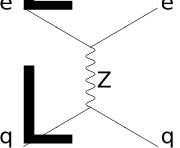
\includegraphics[scale=0.7]{dd}
  \caption{$t$-channel scattering of Weyl fermions}
  \label{fig:ddex}
\end{figure}

We have then the two particle states \eqref{eq:bkqlel}  with distinguishable particles:
\begin{align}
  e_L\to& \xi_e\,& q_L\to \xi_q\,.
\end{align}

We consider the current of a Weyl fermion mediated by $Z^{\mu}$, with a coupling, $a_L$, given by the Lagrangian
\begin{align}
\label{eq:xietaz}
\mathcal{L}=a_L \xi^{\dagger}_{\dot{\alpha}}\left( \overline{\sigma}^{\mu} \right)^{\dot{\alpha}\alpha}\xi_{\alpha} Z_{\mu}\,.
%+b_L \eta^{\alpha} \sigma^{\mu}_{\alpha\dot{\alpha}} \eta^{\dagger\dot{\alpha}} Z_{\mu}
\end{align}


We label the initial (final) momentum as $p_1$, $p_2$ ($p_1'$, $p_2'$) such that
\begin{align}
  m_e=&m_1=m_1'\,,&m_q=&m_2=m_2'\,.
\end{align}


The specific calculation by the scattering mediated by the $Z^{\mu}$ is 
\begin{align}
  S_{fi}=&\frac{\left( -ia_L \right)^{2}}{2!}\sum_{\text{spins}}\int\int \operatorname{d}^4x_1 \operatorname{d}^4x_2
\bcontraction{\,}{Z_{\mu}}{(x_1)}{Z_{\nu}}\,Z_{\mu}(x_1)Z_{\nu}(x_2) \nonumber\\
&\left\langle q_L \left(\mathbf{p}'_2\right),e_L\left(\mathbf{p}'_1\right) \right|
  : \xi^{\dagger}_{e\dot{\alpha}}(x_1)\left( \overline{\sigma}^{\mu} \right)^{\dot{\alpha}\alpha}\xi_{e\alpha}(x_1)\xi^{\dagger}_{q\dot{\beta}}(x_2)\left( \overline{\sigma}^{\nu} \right)^{\dot{\beta}\beta}\xi_{q\beta}(x_2):
 \left| q_L\left(\mathbf{p}_2\right) ,e_L \left(\mathbf{p}_1\right)  \right\rangle \nonumber\\
=&\frac{\left( -ia_L \right)^{2}}{2!}\sum_{\text{spins}}\int\int \operatorname{d}^4x_1 \operatorname{d}^4x_2
D_{\mu\nu} \left( x_1-x_2 \right)\nonumber\\
&\left\langle q_L \left(\mathbf{p}'_2\right),e_L\left(\mathbf{p}'_1\right)\right|
   \xi^{\dagger}_{e\dot{\alpha} -}(x_1)\xi^{\dagger}_{q\dot{\beta}-}(x_2)\left( \overline{\sigma}^{\mu} \right)^{\dot{\alpha}\alpha}\left( \overline{\sigma}^{\nu} \right)^{\dot{\beta}\beta}\xi_{e\alpha +}(x_1)\xi_{q\beta +}(x_2)
 \left| q_L\left(\mathbf{p}_2\right), e_L \left(\mathbf{p}_1\right)\right\rangle. 
\end{align}



By using~\eqref{eq:bkqlel} we have an expression similar to \eqref{eq:finalsfi}
\begin{align}
      S_{fi}
    =&\frac{(2\pi)^4(ia_L)^2\delta^{(4)}\left(p_1+p_2-p_1'-p_2'\right) }{\sqrt{2 E_1'V}\sqrt{2 E_2'V}\sqrt{2 E_1V}\sqrt{2 E_2V}}
 \left[ x^{\dagger}_{e\dot{\alpha}}(\mathbf{p}_1')\left( \overline{\sigma}^{\mu} \right)^{\dot{\alpha}\alpha}x_{e \alpha}(\mathbf{p}_1)  i D_{\mu\nu}\left(p_1-p_1'\right)x^{\dagger}_{q\dot{\beta}}(\mathbf{p}_2') \left( \overline{\sigma}^{\nu} \right)^{\dot{\beta}\beta}x_{q \beta}(\mathbf{p}_2)\right] \nonumber\\
=&\frac{(2\pi)^4(ia_L)^2\delta^{(4)}\left(p_1+p_2-p_1'-p_2'\right) }{\sqrt{2 E_1'V}\sqrt{2 E_2'V}\sqrt{2 E_1V}\sqrt{2 E_2V}}
  \left[ x_e^{\dagger}(\mathbf{p}_1') \overline{\sigma}^{\mu}x_e(\mathbf{p}_1)  i D_{\mu\nu}\left(p_1-p_1'\right)x_q^{\dagger}(\mathbf{p}_2') \overline{\sigma}^{\nu} x_q(\mathbf{p}_2)\right].
\end{align}
In this way
\begin{align}
  \mathcal{M}=&(ia_L)^2 x_e^{\dagger}(\mathbf{p}_1') \overline{\sigma}^{\mu}x_e(\mathbf{p}_1)  i D_{\mu\nu}(t)x_q^{\dagger}(\mathbf{p}_2') \overline{\sigma}^{\nu} x_q(\mathbf{p}_2)
\end{align}
By using
\begin{align}
  iD_{\mu\nu}=\frac{-ig_{\mu\nu}}{t-m_Z^2}
\end{align}
and the identity \eqref{eq:sos}
\begin{align}
\mathcal{M}=&(ia_L)^2 \frac{(-i)}{t-m_Z^2} x^{\dagger}_{e\dot{\alpha}}(\mathbf{p}_1')\left( \overline{\sigma}^{\mu} \right)^{\dot{\alpha}\alpha}x_{e \alpha}(\mathbf{p}_1)  x^{\dagger}_{q\dot{\beta}}(\mathbf{p}_2') \left( \overline{\sigma}_{\mu} \right)^{\dot{\beta}\beta}x_{q \beta}(\mathbf{p}_2) \nonumber\\
=&(ia_L)^2 \frac{(-i)}{t-m_Z^2} x^{\dagger}_{e\dot{\alpha}}(\mathbf{p}_1')\epsilon^{\alpha\beta}\epsilon^{\dot{\alpha}\dot{\beta}}x_{e \alpha}(\mathbf{p}_1)  x^{\dagger}_{q\dot{\beta}}(\mathbf{p}_2')x_{q \beta}(\mathbf{p}_2) \nonumber\\
=&-(ia_L)^2 \frac{(-i)}{t-m_Z^2}\epsilon^{\beta\alpha}x_{e \alpha}(\mathbf{p}_1)x_{q \beta}(\mathbf{p}_2) x^{\dagger}_{e\dot{\alpha}}(\mathbf{p}_1')  x^{\dagger\dot{\alpha}}_{q}(\mathbf{p}_2') \nonumber\\
=&-(ia_L)^2 \frac{(-i)}{t-m_Z^2}x^{\beta}_e(\mathbf{p}_1)x_{q \beta}(\mathbf{p}_2) x^{\dagger}_{e\dot{\alpha}}(\mathbf{p}_1')  x^{\dagger\dot{\alpha}}_{q}(\mathbf{p}_2') \nonumber\\
=&-(ia_L)^2 \frac{(-i)}{t-m_Z^2}x_e(\mathbf{p}_1)x_q(\mathbf{p}_2) x^{\dagger}_e(\mathbf{p}_1')  x^{\dagger}_q(\mathbf{p}_2') \,.
\end{align}
We now can square the amplitude and sum over spins to obtain from \eqref{eq:xxd} and \eqref{eq:trss}
\begin{align}
  \sum_{\text{spins}} |\mathcal{M}|^2=&
  \frac{a_L^4}{\left( t-m_Z^2 \right)^2}
  \sum_{\text{spins}}x_e(\mathbf{p}_1)x_q(\mathbf{p}_2) x^{\dagger}_e(\mathbf{p}_1')  x^{\dagger}_q(\mathbf{p}_2') 
 x_q(\mathbf{p}_2') x_e(\mathbf{p}_1')  x_q^{\dagger}(\mathbf{p}_2)  x_e^{\dagger}(\mathbf{p}_1) \nonumber\\
  =& \frac{a_L^4}{\left( t-m_Z^2 \right)^2} \operatorname{Tr}\left[p_2'\cdot\overline{\sigma} p_1'\cdot\sigma  \right]
  \sum_{\text{spins}}x_e(\mathbf{p}_1)x_q(\mathbf{p}_2)  x_q^{\dagger}(\mathbf{p}_2)  x_e^{\dagger}(\mathbf{p}_1) \nonumber\\
  =& \frac{a_L^4}{\left( t-m_Z^2 \right)^2} \operatorname{Tr}\left[p_2'\cdot\overline{\sigma} p_1'\cdot\sigma  \right]
 \operatorname{Tr}\left[p_2\cdot\sigma  p_1\cdot\overline{\sigma}  \right] \nonumber\\
  =& \frac{4a_L^4}{\left( t-m_Z^2 \right)^2}\left( p_1\cdot p_2 \right)\left( p_1'\cdot p_2' \right).
\end{align}
The products of momentum can be written in terms of the Mandelstam variables~ \eqref{eq:stucs}
\begin{align}
   \sum_{\text{spins}} |\mathcal{M}|^2=& \frac{a_L^4}{\left( t-m_Z^2 \right)^2}\left( s-m_e^2-m_q^2 \right)^2.
\end{align}
The cross section is 
\begin{align}
     \frac{d\sigma}{d\Omega}=&\frac{1}{64\pi^2s}
\frac{\lambda^{1/2}(s,{m_2'}^2,{m_1'}^2)}{\lambda^{1/2}(s,m_2^2,m_1^2)}
\overline{|\mathcal{M}|^2} \nonumber\\
=&\frac{1}{64\pi^2s}\overline{|\mathcal{M}|^2} \nonumber\\
=&\frac{1}{64\pi^2s}\frac{a_L^4}{\left( t-m_Z^2 \right)^2}\left( s-m_e^2-m_q^2 \right)^2 \,.
\end{align}
In the non-relativistic limit
\begin{align}
  t\approx& (m_e-m_e)^2\approx 0\,,& 
  s\approx& (m_e+m_q)^2\,,
\end{align}
and, in this way,
\begin{align}
       \frac{d\sigma}{d\Omega}=&\frac{1}{64\pi^2}\frac{a_L^4}{m_Z^4}\frac{\left( m_e^2+m_q^2+2m_em_q-m_e^2-m_q^2 \right)^2}{(m_e+m_q)^2} \nonumber\\
                    =&\frac{a_L^4}{16\pi^2m_Z^4}\left( \frac{m_em_q}{m_e+m_q} \right)^2\,.
\end{align}

After the final integration we have
\begin{align}
  \label{eq:csdm}
       \sigma(e_L+q_L\to e_L+q_L)
                    =&\frac{a_L^4}{4\pi m_Z^4}\left( \frac{m_em_q}{m_e+m_q} \right)^2\,.
\end{align}


\subsection{Fermionic dark matter with a $Z'$ mediation}
We are now going  to interpret this interaction in the context of dark matter. By following the discussion in~\cite{Cirelli:2013ufw}, given the very low energies involved in dark matter scattering with matter, the relevant degree of fredom to be considered are the nucleons directly.
$\alpha$
The coupling of a vector field ${Z'}_{\mu}$ with the quark current
\begin{align*}
  \mathcal{L}=f_{q}\left[ \left( q_L \right)^{\dagger}\overline{\sigma}^{\mu}q_L+\left( q_R \right)^{\dagger}{\sigma}^{\mu}q_R \right] Z'_{\mu}\,,
\end{align*}
leads to the same vector interaction with the nucleon current
\begin{align*}
  \mathcal{L}=f_{N} \left[\left( N_L \right)^{\dagger}\overline{\sigma}^{\mu}N_L
  +\left( N_R \right)^{\dagger}{\sigma}^{\mu}N_R \right] Z'_{\mu}\,.
\end{align*}
The nucleon charge is obtained by summing over the valence quark of the nucleons. For $N=p,n$ (proton and neutron respectively)
\begin{align}
  \label{eq:fpfn}
  f_p=&2f_u+f_d\,,& f_n=f_u+2f_d\,,
\end{align}
Note that because of the conservation of the vector current, there is no contribution of
sea quarks or gluons to the effective couplings~\cite{Frandsen:2011cg}


Consider the Lagrangian of and Abelian $\operatorname{U}(1)_X$ with
the$X$-charges of the rigth handed components of the standard model
fields denoted with the symbold of the field, e.g,
$F=-q_X \left(  F_L  \right)$ for $F=Q,L$, and
$f=q_X \left( f_R \right) $ for $f=u,d,e$. In addition we have a Dirac
fermion dark matter candidate with
$\chi =q_X \left( \chi_R \right)=q_X \left( \chi_L \right)$. We
define the covariant derivative
$D_{\mu}=\partial_{\mu} -i g' \widehat{X} Z'_{\mu}$, such that
$\widehat{X}\psi=q_{\psi}\psi$. Then the Lagrangian, relevant for direct detection, is
\begin{align*}
  \mathcal{L}=&i \left( \chi_L \right)^{\dagger} \overline{\sigma}^{\mu} D_{\mu} \chi_L
                +i \left( \chi_R \right)^{\dagger} {\sigma}^{\mu} D_{\mu} \chi_R
                -m \left[\left( \chi_L \right)^{\dagger} \chi_R+\left( \chi_R \right)^{\dagger} \chi_L\right]
                \nonumber\\
                &
                + i \left( Q_L \right)^{\dagger} \overline{\sigma}^{\mu} D_{\mu} Q_L
                +i \left( u_R \right)^{\dagger} {\sigma}^{\mu} D_{\mu} u_R
                +i \left( d_R \right)^{\dagger} {\sigma}^{\mu} D_{\mu} d_R
                 \nonumber\\ %-\chi+\chi 
  \supset& g'\chi \left( \chi_L \right)^{\dagger}  \overline{\sigma}^{\mu}\chi_L Z'_{\mu}
           +g'\chi\left( \chi_R \right)^{\dagger} {\sigma}^{\mu}  \chi_R Z'_{\mu}-m \left[\left( \chi_L \right)^{\dagger} \chi_R+
                \left( \chi_R \right)^{\dagger} \chi_L\right] \nonumber\\
  &-g'Q \left( u_L \right)^{\dagger} \overline{\sigma}^{\mu} u_L Z'_{\mu}
    +g'u \left( u_R \right)^{\dagger} {\sigma}^{\mu}  u_R Z'_{\mu}
-g'Q \left( d_L \right)^{\dagger} \overline{\sigma}^{\mu} d_L Z'_{\mu}
  +g'd \left( d_R \right)^{\dagger} {\sigma}^{\mu}  d_R Z'_{\mu}\,.
\end{align*}

We have the identities
\begin{align}
  \left( f_{L} \right)^{\dagger}\overline{\sigma}^{\mu} f_L=&  \frac{1}{2}\left( f_{L} \right)^{\dagger}\overline{\sigma}^{\mu} f_L
                                                        + \frac{1}{2}\left( f_{L} \right)^{\dagger}\overline{\sigma}^{\mu} f_L \nonumber\\
  =&  \frac{1}{2}\left( f_L \right)^{\dagger}\overline{\sigma}^{\mu} f_L+\frac{1}{2}\left( f_R \right)^{\dagger}{\sigma}^{\mu} f_R
     -\left[ \frac{1}{2}\left( f_L \right)^{\dagger}{\sigma}^{\mu} f_L- \frac{1}{2}\left( f_R \right)^{\dagger}\overline{\sigma}^{\mu} f_R \right],
\end{align}
where the first two terms corresponds to the vector part and the term in brackets is the axial part. Similarly
\begin{align}
   \left( f_{R} \right)^{\dagger}{\sigma}^{\mu} f_R  =&  \frac{1}{2}\left( f_L \right)^{\dagger}\overline{\sigma}^{\mu} f_L+\frac{1}{2}\left( f_R \right)^{\dagger}{\sigma}^{\mu} f_R
     +\left[ \frac{1}{2}\left( f_L \right)^{\dagger}{\sigma}^{\mu} f_L- \frac{1}{2}\left( f_R \right)^{\dagger}\overline{\sigma}^{\mu} f_R \right].
\end{align}

Wa are interested only in the vector part of the interaction, hence
\begin{align}
   \mathcal{L}\supset&g'\chi \left[ \left( \chi_L \right)^{\dagger}  \overline{\sigma}^{\mu}\chi_L+\left( \chi_R \right)^{\dagger} {\sigma}^{\mu}  \chi_R \right]  Z'_{\mu}
           -m \left[\left( \chi_L \right)^{\dagger} \chi_R+
  \left( \chi_R \right)^{\dagger} \chi_L\right] \nonumber\\
  &+g'(u-Q)\left[ \frac{1}{2}\left( u_L \right)^{\dagger}\overline{\sigma}^{\mu} u_L+\frac{1}{2}\left( u_R \right)^{\dagger}{\sigma}^{\mu} u_R  \right]
  +g'(d-Q)\left[ \frac{1}{2}\left( d_L \right)^{\dagger}\overline{\sigma}^{\mu} d_L+\frac{1}{2}\left( d_R \right)^{\dagger}{\sigma}^{\mu} d_R  \right]. \nonumber\\
=& g'\chi \left[ \left( \chi_L \right)^{\dagger}  \overline{\sigma}^{\mu}\chi_L+\left( \chi_R \right)^{\dagger} {\sigma}^{\mu}  \chi_R \right]  Z'_{\mu}
           -m \left[\left( \chi_L \right)^{\dagger} \chi_R+
  \left( \chi_R \right)^{\dagger} \chi_L\right] \nonumber\\
  &+f_u\left[ \frac{1}{2}\left( u_L \right)^{\dagger}\overline{\sigma}^{\mu} u_L+\frac{1}{2}\left( u_R \right)^{\dagger}{\sigma}^{\mu} u_R  \right]
  +f_d\left[ \frac{1}{2}\left( d_L \right)^{\dagger}\overline{\sigma}^{\mu} d_L+\frac{1}{2}\left( d_R \right)^{\dagger}{\sigma}^{\mu} d_R  \right].
\end{align}
where
\begin{align}
  f_u=&g'(u-Q)\,,& f_d=& g'(d-Q).
\end{align}

The direct detection can be calculated directly from the low energy Feynman diagrams involving the neutron and the proton
\begin{align}
  \mathcal{L}_N=&g'\chi \left[ \left( \chi_L \right)^{\dagger}  \overline{\sigma}^{\mu}\chi_L+\left( \chi_R \right)^{\dagger} {\sigma}^{\mu}  \chi_R \right]  Z'_{\mu}
           -m \left[\left( \chi_L \right)^{\dagger} \chi_R+
  \left( \chi_R \right)^{\dagger} \chi_L\right] \nonumber\\
  &+f_p\left[ \frac{1}{2}\left( p_L \right)^{\dagger}\overline{\sigma}^{\mu} p_L+\frac{1}{2}\left( p_R \right)^{\dagger}{\sigma}^{\mu} p_R  \right]
  +f_n\left[ \frac{1}{2}\left( n_L \right)^{\dagger}\overline{\sigma}^{\mu} n_L+\frac{1}{2}\left( n_R \right)^{\dagger}{\sigma}^{\mu} n_R  \right], 
\end{align}
where $f_p$ and $f_u$ are given in eq.~\eqref{eq:fpfn}.
%%%
The corresponding Lagrangian for a nucleus $X^A$ with $A$ nucleons and $Z$ protons is the sum of the Lagrangian for the $Z$ protons and the $(A-Z)$ neutrons
\begin{align}
  \mathcal{L}_{X^A}=&g'\chi \left[ \left( \chi_L \right)^{\dagger}  \overline{\sigma}^{\mu}\chi_L+\left( \chi_R \right)^{\dagger} {\sigma}^{\mu}  \chi_R \right]  Z'_{\mu}
           -m \left[\left( \chi_L \right)^{\dagger} \chi_R+
  \left( \chi_R \right)^{\dagger} \chi_L\right] \nonumber\\
  &+\left[ Z f_p + f_n(A-Z) \right]\left[ \frac{1}{2}\left( X^A_L \right)^{\dagger}\overline{\sigma}^{\mu} X^A_L+\frac{1}{2}\left( X^A_R \right)^{\dagger}{\sigma}^{\mu} X^A_R  \right].
\end{align}
Notice
that the factor
$\left[f_p Z + f_n (A-Z)\right]$
is actually a rescaling factor which is introduced for a
consistent comparison with experimental limits which customarily assume $f_p=f_n$~\cite{Arcadi:2017kky}.

%The calculation for the $\xi_L$-$p_L$ is already done and the result reinterpreted from eq.~\eqref{eq:csdm} for both the proton and the neutron.
In this way, from~\eqref{eq:csdm}, we have the dark matter-nucleus
spin-independent cross section~\cite{Feng:2013vod}
\begin{align}
       \hat{\sigma}_A
                    =&\frac{{g'}^2 \chi^2}{4\pi m_{Z'}^4}\left( \frac{m_\chi m_A}{m_\chi+m_A} \right)^2\left[f_p Z + f_n (A-Z)\right]^2\,.
\end{align}
The specific form of the previous equation, depend on the definition and unitis of $f_N$. For example, by redefining
\begin{align}
  f_N'=\frac{1}{16 m_{Z'}^4}f_N\,,
\end{align}
we have~\cite{Yaguna:2016bga}
\begin{align}
       \hat{\sigma}_A
                    =&\frac{4}{\pi}\left( \frac{m_\chi m_A}{m_\chi+m_A} \right)^2\left[f'_p Z + f'_n (A-Z)\right]^2\,.
\end{align}
In particular, the dark matter-proton spin-independent cross
section is given by
\begin{align}
  \sigma_{p}=\frac{4 \mu_{p}^{2}}{\pi} {f'}_{p}^{2}\,,
\end{align}
where
\begin{align}
  \mu_X=\frac{m_{\chi}m_X}{m_{\chi}+m_X}\,.
\end{align}
is the dark matter-nucleus reduced mass.

The direct detection dark matter-nucleon cross section can be written as
\begin{align}
  \sigma_{N}^{\text{SI}}=\sigma_{p} \frac{\sum_{i} \eta_{i} \mu_{A_{i}}^{2}\left[Z+\left(A_{i}-Z\right) f'_{n} / f'_{p}\right]^{2}}{\sum_{i} \eta_{i} \mu_{A_{i}}^{2} A_{i}^{2}}
\end{align}
where $A_i$ are isotopes of the target nucleus $A$ with fractional number abundances $\eta_i$.

Notice that $\sigma_{N}^{\text{SI}}=\sigma_{p}$ for $f_n'=f_p'$, and the details of the nucleous like their mass, isotopes or abundances, are not longer required.


\subsection{Scalar dark matter with vector couplings}

The following calculation is expected to be self-contained with every step worked out in detail.

To have the Higgs portal direct dark matter detection cross section
The relevant term for the scattering that we consider now is the $t$-channel
\begin{align}
  S(p_1)+q_L^{-}(p_2)\to  S(p_1')+q_R^{-}(p_2')
\end{align}

As always, we use the left-handed Weyl spinors
\begin{align}
  q_L\to &\xi_{\alpha}\,, &   \left( q_R \right)^{\dagger}\to &\eta^{\alpha}\,,
\end{align}


We need the interaction of a singlet scalar with the standard model Higgs, $h(x)$, and the standard model Yukawa
\begin{align}
  \mathcal{L}=&\lambda v S^2(x) h(x)+y \left(q_R\right)^{\dagger} q_L(x) h^0 +y \left(q_L\right)^{\dagger} q_R(x) h(x) \nonumber\\
  =&\lambda v S^2(x) h(x)+y \eta^{\alpha} (x)\xi_{\alpha}(x)h(x) + y \eta^{\dagger\dot{\alpha}}(x) \xi_{\dot{\alpha}}^{\dagger}(x)h(x)\,. 
\end{align}

hence
\begin{align}
  \mathcal{H}_{\text{int}}^{S}=&-\lambda v S^2(x) h(x)\,, &
   \mathcal{H}_{\text{int}}^{q}=&-y \eta^{\alpha} (x)\xi_{\alpha}(x)h(x)\,,
\end{align}

The $S$-matrix expansion includes
\begin{align}
S^{(2)}=&  \frac{(-i)^2}{2!}\int\int d^4x_1 d^4x_2\,\operatorname{T}\{\mathcal{H}_{\text{int}}^S(x_1)\mathcal{H}_{\text{int}}^q(x_2)\}\nonumber\\
=&  \frac{(-i)^2}{2!}\lambda y v\int\int d^4x_1 d^4x_2\,\operatorname{T}\{\left(S S h \right)_{x_1} \left( \eta^{\alpha} \xi_{\alpha}h \right)_{x_2}\}\nonumber\\
=& 
 \frac{(-i)^2}{2!}\lambda y v\int\int d^4x_1 d^4x_2\,:( S
\bcontraction{S}{h}{)_{x_1}(\eta^{\alpha} \xi_{\alpha}}{h}
S h)_{x_1}(\eta^{\alpha} \xi_{\alpha}h
)_{x_2}:+\cdots
\end{align}
In this way
\begin{align}
  S^{(2)}(S q\to S q)=&\frac{(-iy)^2}{2!}\int\int d^4x_1 d^4x_2
\bcontraction{\,}{h}{(x_1)}{h}
\,h(x_1)h(x_2):(SS)_{x_1}(\eta^{\beta} \xi_{\beta})_{x_2}:
\end{align}
On the other hand 
\begin{align}
\label{eq:ss156f}
  :(SS)_{x_1}(\eta^{\beta} \xi_{\beta})_{x_2}:=&
:S(x_1) S(x_1) \eta^{\beta}(x_2) \xi_{\beta}(x_2):\,.
\end{align}



We label the initial (final) momentum as $p_1$, $p_2$ ($p_1'$, $p_2'$) such that
\begin{align}
  m_S=&m_1=m_1'\,,&m_q=&m_2=m_2'\,.
\end{align}


The specific calculation by the scattering mediated by the Higgs is 
\begin{align}
  \label{eq:ss32}
  S_{fi}=&\frac{\lambda  v y_q }{2!}\sum_{\text{spins}}\int\int \operatorname{d}^4x_1 \operatorname{d}^4x_2
\bcontraction{\,}{h}{(x_1)}{h}\,h(x_1)h(x_2) \nonumber\\
&\left\langle q_R \left(\mathbf{p}'_2\right),S\left(\mathbf{p}'_1\right) \right|
  : S(x_1)S(x_1)
    \eta^{\beta}\xi_{\beta}(x_2)(x_2):
 \left| q_L\left(\mathbf{p}_2\right) ,S \left(\mathbf{p}_1\right)  \right\rangle \nonumber\\
=&\frac{ \lambda  m_q }{\sqrt{2}}\sum_{\text{spins}}\int\int \operatorname{d}^4x_1 \operatorname{d}^4x_2
\,i\Delta_F \left( x_1-x_2 \right)\nonumber\\
&\qquad\times\left\langle q_R \left(\mathbf{p}'_2\right),S\left(\mathbf{p}'_1\right)\right|
   S_-(x_1)\eta^{\beta}_{-}(x_2) S_+(x_1)\xi_{\beta +}(x_2)
 \left| q_L\left(\mathbf{p}_2\right), S \left(\mathbf{p}_1\right)\right\rangle. 
\end{align}

where $m_q=y_d v/\sqrt{2}$. This means that $S(\mathbf{p}_1)$ ($q_L(\mathbf{p}_2)$) is destroyed in $x_1$ ($x_2$), while
$S(\mathbf{p}_1')$ ($q_L(\mathbf{p}_2')$) is created in $x_1$ ($x_2$).


When the two particles are distinguishable: For example if the spin of $q_L$ is $s_2$ and $s'$, then %recalculate
\begin{align}
  S_{+}(x_1)&\xi_{\beta +}(x_2)|q_L(\mathbf{p}_2)S(\mathbf{p}_1)\rangle= \nonumber\\
&\int\frac{\operatorname{d}^3k}{(2\pi)^3\sqrt{2E_k V}}a(\mathbf{k})\int\frac{\operatorname{d}^3k'}{(2\pi)^3\sqrt{2E_{k'}V}} 
           x_\beta(s',\mathbf{k}')a_{s'}(\mathbf{k}')\operatorname{e}^{-i k\cdot x_1}\operatorname{e}^{-i k'\cdot x_2} \left| q_L\left(\mathbf{p}_2\right), S \left(\mathbf{p}_1\right)\right\rangle\\ \nonumber
\end{align}

The two particle Fock state is, after proper normalization
\begin{align}
  |q_L(\mathbf{p}_2)S(\mathbf{p}_1)\rangle=&\frac{1}{\sqrt{V^2}}a^\dagger(\mathbf{p}_1)a_{s_2}^\dagger(\mathbf{p}_2)|0\rangle.
\end{align}
Therefore
\begin{align}
  S_{+}(x_1)\xi_{\beta +}(x_2)|q_L(\mathbf{p}_2)S(\mathbf{p}_1)\rangle   =&
\int\frac{\operatorname{d}^3k}{(2\pi)^3\sqrt{2E_k V}}\int\frac{\operatorname{d}^3k'}{(2\pi)^3\sqrt{2E_{k'}V}}
x_\beta(s',\mathbf{k}')\operatorname{e}^{-i k\cdot x_1}\operatorname{e}^{-i k'\cdot x_2}\nonumber\\
&\times a(\mathbf{k})a_{s'}(\mathbf{k}')a^\dagger(\mathbf{p}_1)a_{s_2}^\dagger(\mathbf{p}_2)|0\rangle \nonumber\\
=&
\int\frac{\operatorname{d}^3k'}{(2\pi)^3\sqrt{2E_k V}}\int\frac{\operatorname{d}^3k}{(2\pi)^3\sqrt{2E_{k'}V}}
x_\beta(s',\mathbf{k}')\operatorname{e}^{-i k\cdot x_1}\operatorname{e}^{-i k'\cdot x_2}\nonumber\\
&\times \left[ a(\mathbf{k})a_{s'}(\mathbf{k}')a^\dagger(\mathbf{p}_1)a_{s_2}^\dagger(\mathbf{p}_2) - a^\dagger(\mathbf{p}_1)a_{s_2}^\dagger(\mathbf{p}_2) a(\mathbf{k})a_{s'}(\mathbf{k}') \right]|0\rangle \nonumber\\
=&
\int\frac{\operatorname{d}^3k}{(2\pi)^3\sqrt{2E_k V}}\int\frac{\operatorname{d}^3k'}{(2\pi)^3\sqrt{2E_{k'}V}}
x_\beta(s',\mathbf{k}')\operatorname{e}^{-i k\cdot x_1}\operatorname{e}^{-i k'\cdot x_2}\nonumber\\
&\times \left[ a(\mathbf{k})a_{s'}(\mathbf{k}'),a^\dagger(\mathbf{p}_1)a_{s_2}^\dagger(\mathbf{p}_2)\right]|0\rangle.
\end{align}
By using the identity
\begin{align}
  [AB,CD]=A[B,C]D - [A,C]BD
+CA[B, D] - C[A, D]B\,,
\end{align}
\begin{align}
   \left[ a(\mathbf{k})a_{s'}(\mathbf{k}'),a^\dagger(\mathbf{p}_1)a_{s_2}^\dagger(\mathbf{p}_2)\right]=&
 a(\mathbf{k})\cancel{\left[ a_{s'}(\mathbf{k}'),a^\dagger(\mathbf{p}_1)\right]}a_{s_2}^\dagger(\mathbf{p}_2)
-
 \left[ a(\mathbf{k}),a^\dagger(\mathbf{p}_1)\right]a_{s'}(\mathbf{k}')a_{s_2}^\dagger(\mathbf{p}_2) \nonumber\\
& 
+a^\dagger(\mathbf{p}_1)a(\mathbf{k})\left[ a_{s'}(\mathbf{k}'),a_{s_2}^\dagger(\mathbf{p}_2)\right]
-
a^\dagger(\mathbf{p}_1) \cancel{\left[ a(\mathbf{k}),a_{s_2}^\dagger(\mathbf{p}_2)\right]}a_{s'}(\mathbf{k}') \nonumber\\
=&
-
 \left[ a(\mathbf{k}),a^\dagger(\mathbf{p}_1)\right]a_{s'}(\mathbf{k}')a_{s_2}^\dagger(\mathbf{p}_2)  
+\left[ a_{s'}(\mathbf{k}'),a_{s_2}^\dagger(\mathbf{p}_2)\right]a^\dagger(\mathbf{p}_1)a(\mathbf{k})
\end{align}
Therefore,
\begin{align}
&\left[ a(\mathbf{k})a_{s'}(\mathbf{k}'),a^\dagger(\mathbf{p}_1)a_{s_2}^\dagger(\mathbf{p}_2)\right] |0\rangle \nonumber\\
&\qquad=
-
 \left[ a(\mathbf{k}),a^\dagger(\mathbf{p}_1)\right]a_{s'}(\mathbf{k}')a_{s_2}^\dagger(\mathbf{p}_2) |0\rangle \nonumber\\
&\qquad=-
  \left[ a(\mathbf{k}),a^\dagger(\mathbf{p}_1)\right] \left[ a_{s'}(\mathbf{k}'),a_{s_2}^\dagger(\mathbf{p}_2)  \right] |0\rangle \nonumber\\
&\qquad= -(2\pi)^6  
    \delta^{(3)}(\mathbf{k}-\mathbf{p}_1)\delta^{(3)}(\mathbf{k}'-\mathbf{p}_2)|0\rangle
\end{align}
and
\begin{align}
\label{eq:ssbkqlel}
S_{+}(x_1)\xi_{\beta +}(x_2)|q_L(\mathbf{p}_2)S(\mathbf{p}_1)\rangle  =&
 -\frac{1}{\sqrt{2E_1 V}\sqrt{2E_2 V}}\,x_{\beta}(s',\mathbf{p}_2)\operatorname{e}^{-i p_1\cdot x_1}\operatorname{e}^{-i p_2\cdot x_2}|0\rangle\,.
\end{align}

Following similar steps, we find
\begin{align}
\label{eq:ssberer}
  S_{+}(x_1)& \eta^{\dagger\dot{\beta}}_{+}(x_2)|q_R(\mathbf{p}_2)S(\mathbf{p}_1')\rangle
 =-\frac{1 }{\sqrt{2 E_1'V}\sqrt{2 E_2'V}}  y^{\dagger\dot{\beta}}(s',\mathbf{p}_2')
 \operatorname{e}^{-i p'_1\cdot x_1}\operatorname{e}^{-i p'_2\cdot x_2}\left|0\right\rangle \\
  \langle q_R(\mathbf{p}_2')&S(\mathbf{p}_1')| S_{-}(x_1)\eta^{\beta}_{-}(x_2)
 =-\left\langle 0\right|\frac{1 }{\sqrt{2 E_1'V}\sqrt{2 E_2'V}}  y^{\beta}(s',\mathbf{p}_2')
 \operatorname{e}^{i p'_1\cdot x_1}\operatorname{e}^{i p'_2\cdot x_2}\,.
\end{align}

Hence
\begin{align}
  \langle q_R(\mathbf{p}_2')&S(\mathbf{p}_1')| S_{-}(x_1)\eta^{\beta}_{-}(x_2)
  S_{+}(x_1)\xi_{\beta +}(x_2)|q_L(\mathbf{p}_2)S(\mathbf{p}_1)\rangle \nonumber\\
=&\left\langle 0\right|\frac{1 }{\sqrt{2 E_1'V}\sqrt{2 E_2'V}}  y^{\beta}(s',\mathbf{p}_2')
   \operatorname{e}^{i p_1'\cdot x_1}\operatorname{e}^{i p_2'\cdot x_2}
\frac{1}{\sqrt{2E_1 V}\sqrt{2E_2 V}}\,x_{\beta}(s',\mathbf{p}_2)\operatorname{e}^{-i p_1\cdot x_1}\operatorname{e}^{-i p_2\cdot x_2}|0\rangle \nonumber\\
=&\frac{1}{\sqrt{2E_1 V}\sqrt{2E_2 V}}\frac{1 }{\sqrt{2 E_1'V}\sqrt{2 E_2'V}}  y^{\beta}(s',\mathbf{p}_2')\,x_{\beta}(s',\mathbf{p}_2)
   \operatorname{e}^{i p_1'\cdot x_1}\operatorname{e}^{i p_2'\cdot x_2}
\operatorname{e}^{-i p_1\cdot x_1}\operatorname{e}^{-i p_2\cdot x_2}\langle 0|0\rangle \nonumber\\
=&\frac{1}{\sqrt{2E_1 V}\sqrt{2E_2 V}}\frac{1 }{\sqrt{2 E_1'V}\sqrt{2 E_2'V}}  y^{\beta}(s',\mathbf{p}_2')\,x_{\beta}(s',\mathbf{p}_2)
   \operatorname{e}^{i p_1'\cdot x_1}\operatorname{e}^{i p_2'\cdot x_2}
\operatorname{e}^{-i p_1\cdot x_1}\operatorname{e}^{-i p_2\cdot x_2}\,.
\end{align}

Checking back eq.~\eqref{eq:ss32}, we see that 
\begin{align}
  \label{eq:ss37}
S_{fi}=&\frac{ \lambda  m_q }{\sqrt{2}}\frac{1}{\sqrt{2E_1 V}\sqrt{2E_2 V}}\frac{1 }{\sqrt{2 E_1'V}\sqrt{2 E_2'V}}  y^{\beta}(s',\mathbf{p}_2')\,x_{\beta}(s',\mathbf{p}_2)\sum_{\text{spins}} \mathcal{I}\,,
\end{align}
where
\begin{align}
  \mathcal{I}=\int\int \operatorname{d}^4x_1 \operatorname{d}^4x_2
\,i\Delta_F \left( x_1-x_2 \right)   \operatorname{e}^{i p_1'\cdot x_1}\operatorname{e}^{i p_2'\cdot x_2}
\operatorname{e}^{-i p_1\cdot x_1}\operatorname{e}^{-i p_2\cdot x_2}\,.
\end{align}
The integral is easily eavaluated if we use the Fourier expansion
\begin{align}
  i\Delta_F \left( x_1-x_2 \right)=
  \int \frac{\operatorname{d}^4q}{\left( 2\pi \right)^4} i \Delta(q)
  \operatorname{e}^{iq\cdot(x_1-x_2)}\,,
\end{align}
such that
\begin{align}
   \mathcal{I}=&\int\int \operatorname{d}^4x_1 \operatorname{d}^4x_2
\,i\Delta_F \left( x_1-x_2 \right)   \operatorname{e}^{i p_1'\cdot x_1}\operatorname{e}^{i p_2'\cdot x_2}
\operatorname{e}^{-i p_1\cdot x_1}\operatorname{e}^{-i p_2\cdot x_2} \nonumber\\
=&  \int \frac{\operatorname{d}^4q}{\left( 2\pi \right)^4} i \Delta(q)
\int\int \operatorname{d}^4x_1 \operatorname{d}^4x_2
\, \operatorname{e}^{iq\cdot(x_1-x_2)}    \operatorname{e}^{i p_1'\cdot x_1}\operatorname{e}^{i p_2'\cdot x_2}
\operatorname{e}^{-i p_1\cdot x_1}\operatorname{e}^{-i p_2\cdot x_2}   
\end{align}

\begin{align}
  =& \left( 2\pi \right)^4 \int {\operatorname{d}^4q}\, i \Delta(q)
\int\int \frac{\operatorname{d}^4x_1}{\left( 2\pi \right)^4} \frac{\operatorname{d}^4x_2}{\left( 2\pi \right)^4} 
\, \operatorname{e}^{-i(-q-p_1'+p_1)\cdot x_1}   
\, \operatorname{e}^{-i(q-p_2'+p_2)\cdot x_2}   \nonumber\\
 =& \left( 2\pi \right)^4 \int {\operatorname{d}^4q}\, i \Delta(q)
\, \delta^{4}(-q-p_1'+p_1)   
\, \delta^4(q-p_2'+p_2).
\end{align}
By using the first  $\delta$-function to make the final integration on $q$, we have
\begin{align}
  \mathcal{I} =& \left( 2\pi \right)^4 \, i \Delta(p_1-p_1')   
\, \delta^4(p_1+p_2-p_1'-p_2') \,.
\end{align}
Replacing back in eq.~\eqref{eq:ss37}
\begin{align}
      S_{fi}
    =&\frac{(2\pi)^4 \lambda m_q \delta^{(4)}\left(p_1+p_2-p_1'-p_2'\right) }{\sqrt{2 E_1'V}\sqrt{2 E_2'V}\sqrt{2 E_1V}\sqrt{2 E_2V}}
 \left[y^{\prime\beta}_2\,i\Delta_F(p_1-p_1')x_{2\beta}\right] \nonumber\\
\end{align}
where
\begin{align}
  y^{\prime\beta}_2\equiv&   y^{\beta}(s',\mathbf{p}_2'), &
  x_{2\beta}\equiv&   x_{\beta}(s',\mathbf{p}_2).                           
\end{align}
Comparing with the general expression for the $2\to 2$ processes, we get that

\begin{align}
 i\mathcal{M}=\lambda  m_q\Delta_F(p_1-p_1')y^{\prime \alpha}_2 x_{2\alpha}\,.
\end{align}
As an initial step to calculate the probability we must squared this amplitude
\begin{align}
  \sum_{\text{spins}} |\mathcal{M}|^2=&\lambda^2   m_q^2\Delta_F^2(p_1-p_1')
     \sum_{\text{spins}} y^{\prime \alpha}_2 x_{2\alpha}x^{\dagger}_{2\dot{\alpha}} y^{\prime\dagger\dot{\alpha}}_2     \nonumber\\
=&\lambda^2   m_q^2\Delta_F^2(p_1-p_1')
     \sum_{\text{spins}}  x_{2\alpha}x^{\dagger}_{2\dot{\alpha}} y^{\prime\dagger\dot{\alpha}}_2 y^{\prime \alpha}_2     \nonumber\\
=&\lambda^2   m_q^2\Delta_F^2(p_1-p_1')
   \left( p_2\cdot \sigma \right)_{\alpha\dot{\alpha}} \left( p_2'\cdot \overline{\sigma} \right)^{\dot{\alpha}\alpha}      \nonumber\\
  =& 2 \lambda^2 m_q^2\Delta_F^2(p_1-p_1') \operatorname{Tr}\left( p_2\cdot \sigma p_2'\cdot \overline{\sigma} \right) \nonumber\\
  =& 2 \lambda^2 m_q^2\Delta_F^2(p_1-p_1') \operatorname{Tr}\left( p_2^{\mu} \sigma_{\mu} p_2^{\prime \nu} \overline{\sigma}_{\nu} \right) \nonumber\\
  =& 2 \lambda^2 m_q^2\Delta_F^2(p_1-p_1')\operatorname{Tr}\left(  \sigma_{\mu}  \overline{\sigma}_{\nu} \right) p_2^{\mu} p_2^{\prime \nu}\nonumber\\
  =& 4 \lambda^2 m_q^2\Delta_F^2(p_1-p_1') g_{\mu\nu} p_2^{\mu} p_2^{\prime \nu}\nonumber\\
  =& 4 \lambda^2 m_q^2\Delta_F^2(p_1-p_1') \left( p_2\cdot p_2' \right) 
\end{align}

The partial amplitude can be written in terms of the Mandelstam variables~\eqref{eq:mvstu} and \eqref{eq:stucs}
\begin{align}
  \sum_{\text{spins}} |\mathcal{M}|^2
  =& 4 \lambda^2 m_q^2\Delta_F^2(p_1-p_1') 
     \left( m_2^2+{m_2'}^2-t \right),
\end{align}
where
\begin{align}
  t=\left( p_1-p_1' \right)^2=\left( p_2-p_2' \right)^2\,.
\end{align}

By using
\begin{align}
  i\Delta_F( p_1-p_1')=\frac{-i}{(p_1-p_1')^2-m_h^2}
  =\frac{-i}{t-m_h^2}\,,
\end{align}
and, since $m_S=m_1=m_1'$, $m_q=m_2=m_2'$
\begin{align}
   \sum_{\text{spins}} |\mathcal{M}|^2=&\frac{\lambda^2 m_q^2}{\left( t-m_h^2 \right)^2} \left(2m_q^2-t\right).
\end{align}
Therefore
\begin{align}
     \frac{d\sigma}{d\Omega}=&\frac{1}{64\pi^2s}
\frac{\lambda^{1/2}(s,{m_2'}^2,{m_1'}^2)}{\lambda^{1/2}(s,m_2^2,m_1^2)}
                               \overline{|\mathcal{M}|^2} \nonumber\\
=&\frac{1}{64\pi^2s}\left\{
\frac{[s-(m_1'+m_2')^2][s-(m_1'-m_2')^2]}{[s-(m_1+m_2)^2][s-(m_1-m_2)^2]}\right\}^{1/2}
\overline{|\mathcal{M}|^2}  
\end{align}
\begin{align}
  =&\frac{1}{64\pi^2s}\left\{
\frac{[s-(m_S+m_q)^2][s-(m_S-m_q)^2]}{[s-(m_S+m_q)^2][s-(m_S-m_q)^2]}\right\}^{1/2}
\overline{|\mathcal{M}|^2}  
\end{align}
And we have 
\begin{align}
\frac{d\sigma}{d\Omega}  =&\frac{1}{64\pi^2s}\overline{|\mathcal{M}|^2} \nonumber\\
  =&\frac{1}{64\pi^2s}\frac{\lambda^2 m_q^2}{\left( t-m_h^2 \right)^2}
     \left(2m_q^2-t\right).
\end{align}

In the non-relativistic limit
\begin{align}
  t\approx& (m_S-m_S)^2\approx 0\,,& 
  s\approx& (m_S+m_q)^2\,,
\end{align}
\begin{align}
   \frac{d\sigma}{d\Omega}=& \frac{\lambda^2 m_q^4}{32\pi^2 \left(m_S+m_q\right)^2m_h^4}\nonumber\\
  =&
     \frac{\lambda^2 m_q^4}{32\pi^2 m_h^4\left(m_S+m_q\right)^2}
     \frac{m_S^2}{m_S^2}\nonumber\\
       \frac{d\sigma}{d\Omega}
                    =&\frac{\lambda^2m_q^2}{32\pi^2m_h^4m_S^2}\left( \frac{m_Sm_q}{m_S+m_q} \right)^2\,.
\end{align}


\subsection{Fermion dark matter with scalar couplings}

\begin{frame}[fragile,allowframebreaks]
We repeat here the calculation of the Higgs mediated scattering in sec.~\ref{sec:higgs-medi-scatt} but for the explicit case of distinguishable particles. To be more specific, 
we now consider the $t$-channel interaction
\begin{align}
  e_L+q_L \to e_R+q_R\,,
\end{align}
mediated by $h(x)$, with couplings
\begin{align}
\label{eq:xietaz}
\mathcal{L}= y_e \left(e_R\right)^{\dagger} e_L h^0 +y \left(e_L\right)^{\dagger} e_R h^0 
+y_q \left(q_R\right)^{\dagger} q_L h^0 +y \left(q_L\right)^{\dagger} q_R h^0 \,.
\end{align}


The specific calculation by the scattering mediated by the Higgs, $h(x)$, is 
\begin{align}
  S_{fi}=&\frac{\left(y_ey_q \right)}{2!}\sum_{\text{spins}}\int\int \operatorname{d}^4x_1 \operatorname{d}^4x_2
\bcontraction{\,}{h}{(x_1)}{h}\,h(x_1)h(x_2) \nonumber\\
&\left\langle q_R \left(\mathbf{p}'_2\right),e_R\left(\mathbf{p}'_1\right) \right|
  : \xi^{\alpha}_{e}(x_1)\eta_{e\alpha}(x_1)
    \xi^{\beta}_{q}(x_2)\eta_{q\beta}(x_2):
 \left| q_L\left(\mathbf{p}_2\right) ,e_L \left(\mathbf{p}_1\right)  \right\rangle \nonumber\\
=&\frac{\left( y_ey_d \right)}{2!}\sum_{\text{spins}}\int\int \operatorname{d}^4x_1 \operatorname{d}^4x_2
i\Delta_F \left( x_1-x_2 \right)\nonumber\\
&\left\langle q_R \left(\mathbf{p}'_2\right),e_R\left(\mathbf{p}'_1\right)\right|
   \eta_{e\alpha-}(x_1)\eta_{q\beta-}(x_2) \xi^{\alpha}_{e+}(x_1)\xi^{\beta}_{q+}(x_2)
 \left| q_L\left(\mathbf{p}_2\right), e_L \left(\mathbf{p}_1\right)\right\rangle. 
\end{align}



By using the standard procedure
\begin{align}
      S_{fi}
    =&\frac{(2\pi)^4y_e y_q \delta^{(4)}\left(p_1+p_2-p_1'-p_2'\right) }{\sqrt{2 E_1'V}\sqrt{2 E_2'V}\sqrt{2 E_1V}\sqrt{2 E_2V}}
 \left[y'_{1\alpha}y'_{2\beta}i\Delta_F(p_1-p_1')x_1^{\alpha}x_2^{\beta}\right] \nonumber\\
\end{align}
\begin{align}
 i\mathcal{M}=y_e y_q\Delta_F(t) x_1y'_1x_2y'_2 
\end{align}
\begin{align}
\sum_{\text{spins}} |\mathcal{M}|^2=&y_e y_q\Delta_F(t) \sum_{\text{spins}}  x_1y'_1x_2y'_2  y^{\prime\dagger}_2x_2^{\dagger} y^{\prime\dagger}_1x^{\dagger}_1 \nonumber\\
=& 4 y_e y_q\Delta_F(t) \left( p_2\cdot p_2' \right) \left(p_1\cdot p_1'  \right)
\end{align}
By using
\begin{align}
  i\Delta_F(t)=\frac{-i}{t-m_h^2}
\end{align}
Since $m_e=m_1=m_1'$, $m_q=m_2=m_2'$
\begin{align}
   \sum_{\text{spins}} |\mathcal{M}|^2=&\frac{y_ey_q}{\left( t-m_h^2 \right)^2} \left(2m_e^2-t\right)\left(2m_q^2-t\right)
\end{align}
\begin{align}
     \frac{d\sigma}{d\Omega}=&\frac{1}{64\pi^2s}
\frac{\lambda^{1/2}(s,{m_2'}^2,{m_1'}^2)}{\lambda^{1/2}(s,m_2^2,m_1^2)}
\overline{|\mathcal{M}|^2} \nonumber\\
=&\frac{1}{64\pi^2s}\overline{|\mathcal{M}|^2} \nonumber\\
=&\frac{1}{64\pi^2s}\frac{y_e^2y_q^2}{\left( t-m_h^2 \right)^2}\left(2m_e^2-t\right)\left(2m_q^2-t\right) .
\end{align}
In the non-relativistic limit
\begin{align}
  t\approx& (m_e-m_e)^2\approx 0\,,& 
  s\approx& (m_e+m_q)^2\,,
\end{align}
\begin{align}
       \frac{d\sigma}{d\Omega}
                    =&\frac{y_e^2y_q^2}{16\pi^2m_h^4}\left( \frac{m_em_q}{m_e+m_q} \right)^2 \nonumber\\
=&\frac{m_e^2m_q^2}{16\pi^2v^4 m_h^4}\left( \frac{m_em_q}{m_e+m_q} \right)^2\,,
\end{align}
where $m_f=y_f v$.

\section{Relic density}
\subsection{Vector portal}
See full treatment in \url{https://indico.cern.ch/event/746178/contributions/3384110/attachments/1849289/3035359/SUSY2019_SatomiOkada.pdf}

\end{frame}

\section{Extra examples}
Solved problems in~\cite{Maggiore:2005qv} 
\begin{itemize}
\item  $\pi^+\to l^+\nu_l $ (Problem 8.2, pag. 205)
\end{itemize}

\section{Exercises}
Display possible diagrams that correct the mass of the scalar in a theory with $\lambda \phi^4$, with and without a $\phi^3$-term.




%%% Local Variables: 
%%% mode: latex
%%% TeX-master: "beyond"
%%% End: